\section{Global terrestrial carbon fluxes estimates} \label{chap4_s2}
% \renewcommand{\headrulewidth}{0pt}
% \lhead[\thepage]{\leftmark}
% \rhead[\leftmark]{\thepage}
% \cfoot[]{}

\subsection{Background and summary}
Terrestrial ecosystems play a crucial role in mitigating global warming by serving as a persistent carbon sink, actively absorbing and storing excess carbon dioxide from the atmosphere \citep{pan2011large}. Over the period from 2010 to 2019, the terrestrial CO\textsubscript{2} sink is estimated to offset fossil CO\textsubscript{2} emissions by 35\%, surpassing the ocean, which is projected to remove 26\% of fossil-fuel-derived CO\textsubscript{2} \citep{friedlingstein2020global, wang2022disentangling}. The substantial global carbon flux, known as terrestrial gross primary production (GPP), significantly contributes to the reduction of anthropogenic CO\textsubscript{2} emissions \citep{beer2010terrestrial}. \par

Estimating GPP involves various methods, such as simulating dynamic global vegetation models (DGVMs) like those employed in the TRENDY project \citep{sitch2015recent, le2018global}, upscaling from measurements obtained through eddy covariance (EC) flux tower and satellite observations \citep{jung2019fluxcom, zeng2020global}. However, all these approaches rely on plant functional types (PFTs) to estimate ecosystem productivity \citep{poulter2011plant, poulter2015plant, lin2021improved, guo2023estimating, yan2023integrating}. Inconsistencies in PFT maps can significantly contribute to uncertainties in GPP estimations, as well as other climate-relevant variables, at both regional and global scales \citep{poulter2011plant}. Particularly in the tropical region, the sparse distribution of EC sites, the high species richness of trees, and the complex vertical structure of tropical rainforests pose challenges \citep{montgomery2001forest}, making it difficult to accurately quantify the seasonality of carbon fluxes \citep{xu2015satellite}. \par

In recent times, there has been an increasing adoption of timeseries (TS) foundation models employing a transformer-inspired architecture for addressing timeseries problems and representation learning. Notable examples include the MVTS Transformer \citep{zerveas2021transformer}, Informer \citep{zhou2021informer}, Autoformer \citep{wu2021autoformer}, and Fedformer \citep{zhou2022fedformer}. The adoption of the Transformer architecture is anticipated to enhance the modeling of seasonality based on the timeseries representation. However, to the best of our knowledge, its application in the task of upscaling global carbon fluxes remains limited. \par

In this chapter, our goal is to evaluate the effectiveness of employing timeseries representation, specifically based on recently updated Plant Functional Types (PFTs) \citep{harper202229} and a Transformer-based architecture model \citep{zerveas2021transformer}, for predicting the trends and seasonality of carbon fluxes at a global scale. We present monthly global data at a spatial resolution of 0.25 degrees for GPP and Ecosystem Respiration (RECO). The evaluation of our dataset involves comparing it with other satellite-based carbon flux datasets, considering correlations with FLUXNET 2015 and Solar-Induced Fluorescence (SIF) datasets, as well as assessing interannual trends and variations. The overall workflow of the study is depicted in \ref{fig:chap6_fig1}.

\begin{figure}[tbh!]
    \centering
    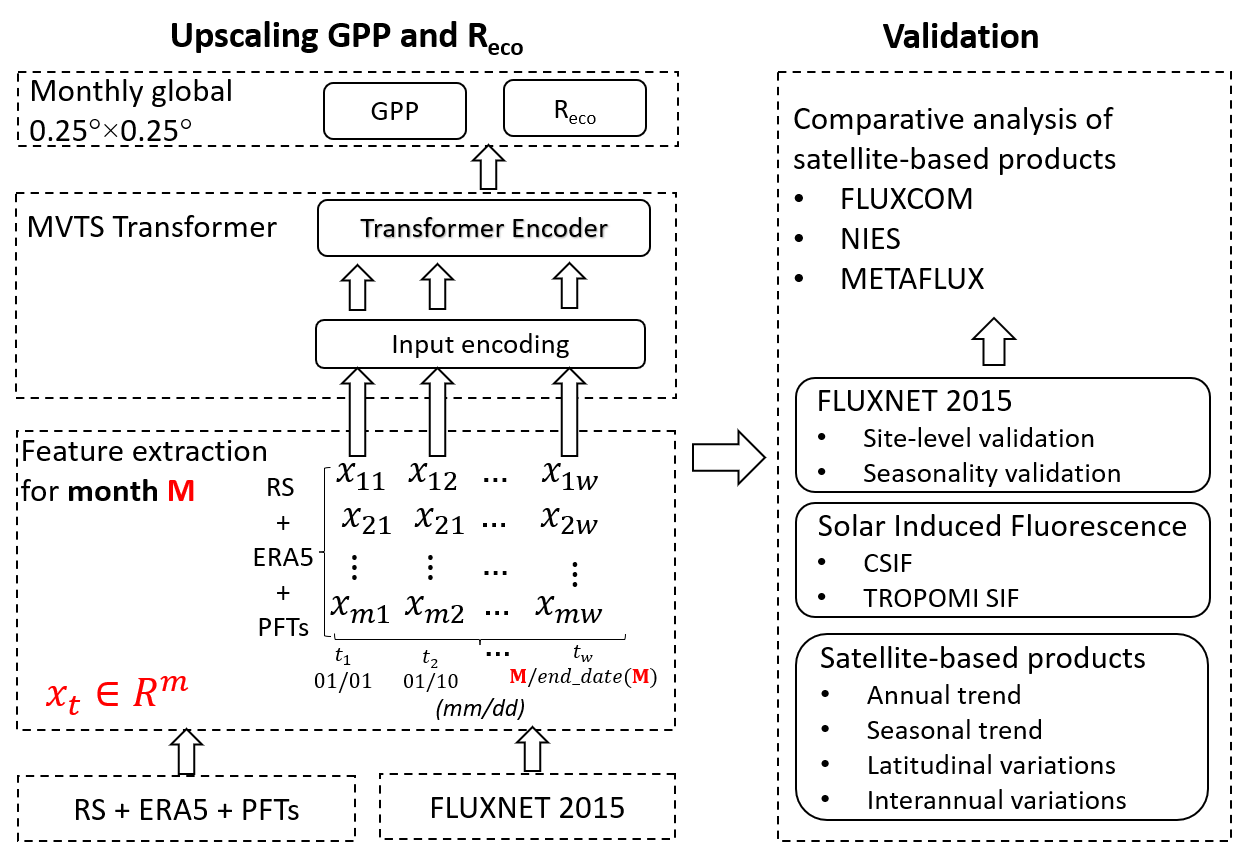
\includegraphics[width=\textwidth]{figs/chap6/workflow.png}
    \caption[Schemantic workflow of our FluxFormer methodology]{Schemantic workflow of our FluxFormer methodology}
    \label{fig:chap6_fig1}
\end{figure}

\subsection{Methods}
\subsubsection*{Input data}

\paragraph*{FLUXNET 2015}
The FLUXNET 2015 dataset \citep{pastorello2020fluxnet2015} serves as the groundtruth for carbon fluxes in the transformer model in this study. Monthly GPP and RECO data were extracted from the dataset tier 1 of FLUXNET 2015, encompassing data from 206 sites. We filtered out records with a quality control value of less than 80\% for measured and good-quality gap-fill data. Relying solely on quality control values is reported to be insufficient for obtaining qualified data due to inconsistencies in the differences between GPP, RECO, and NEE \citep{zeng2020global, tramontana2016predicting}. Following the approach of \citep{zeng2020global}, we also excluded records with an absolute difference between GPP-RECO and NEE larger than 0.1 gC $m^{-2} d^{-1}$.
\paragraph*{Remote sensing data}
For the remote sensing data, we employed version 2 of the global leaf area index (LAI) and fraction of absorbed photosynthetically active radiation (FAPAR) datasets, generated using the algorithm proposed by \citep{verger2014near}. These datasets can be accessed through the Copernicus Global Land Service, providing a 1 km spatial resolution for every 10 days spanning from 1999 to 2019. The remote sensing data utilized in this study is in line with the approach presented in \citep{zeng2020global}. The latitude boundary of this dataset ranges from -60°S to 80°N. \par
\paragraph*{Meteorological data}
For meteorological data, we employed specific variables from the ERA5 reanalysis product \citep{hersbach2020era5}, including 2-meter air temperature (T2M), surface short-wave (solar) radiation downwards (SSRD), vapor pressure deficit (VPD), total precipitation (TP), and evaporation (E). As VPD is not directly available in the original dataset, we estimated it using the relationship between saturated vapor pressure (SVP) and actual vapor pressure (AVP): VPD = SVP - AVP, based on 2-meter air and dewpoint temperature. The original spatial resolution of ERA5 data is 0.25° × 0.25° and was obtained from the Copernicus Climate Change Service (C3S) Climate Data Store (CDS). \par

\paragraph*{Plant function types}
The PFTs dataset employed in this study, denoted as PFT v2.0.8 and obtained from \citep{harper202229}, spans the period from 1992 to 2020. It provides the specific percentage cover of 14 PFTs for each pixel at a 300m resolution. The annual dataset comprises 14 layers, with pixel values at 300m resolution indicating the percentage cover (ranging from 0\% to 100\%) for each of the 14 PFTs. This updated PFTs dataset is considered a more accurate representation of PFT distributions as it relies on high-resolution, peer-reviewed mapping of specific vegetation classes to refine global assumptions about PFT fractions \citep{harper202229}. Regional updates in PFT fractions are anticipated to enhance carbon fluxes estimation. The complete set of PFTs includes bare soil, built areas, water bodies, snow and ice, natural grasses, managed grasses (i.e., herbaceous cropland), broadleaved deciduous trees, broadleaved evergreen trees, needleleaved deciduous trees, needleleaved evergreen trees, broadleaved deciduous shrubs, broadleaved evergreen shrubs, needleleaved deciduous shrubs, and needleleaved evergreen shrubs. The dataset can be accessed from the CEDA archive at https://catalogue.ceda.ac.uk/uuid/26a0f46c95ee4c29b5c650b129aab788.\par

\subsubsection*{Multivariate Time Series Transformer Framework}
Figure \ref{fig:chap6_fig1} illustrates the overall workflow of our FluxFormer methodology to upscale GPP and RECO from remote sensing data, and PFTs data. We utlized the original Multivariate Time Series MVTS Transformer model which is transformer-based framework proposed by \citep{zerveas2021transformer} which contains an input encoding layer with learnable positional encoding and a Transformer Encoder \citep{vaswani2017attention}. MVTS Transformer achieved good performance on supervised and unsupervised regression task based on multivariate time series representation even with limited training samples.  \par
In order train the MVTS Transformer, first, we extracted the remote sensing data, meteorological data and PFTs for each monthly record from FLUXNET 2015 dataset. Then the extracted data is formed to feed to the deep learning model. In particular, for a specific month \textbf{M}, each traing sample $\mathbf{X} \in \mathbb{R}^{w\times n}$ where \textit{w} is the lengths of timeseries for month \textbf{M} $\textit{w} = 3\times \textbf{M}$ as we have three remote sensing products per month and \textit{m} is the number of different variables  $\textit{m} = 21$ 2 remote sensing varibales (LAI and FAPAR), 5 meteorological variables (T2M, SSRD, VPD, TP, E) and 14 PFTs variables, constitutes a sequence of \textit{w} feature vectors $\mathbf{x}\textsubscript{t} \in \mathbb{R}^{m}: \mathbf{X} \in \mathbb{R}^{w\times n} = [\mathbf{x}\textsubscript{1},\mathbf{x}\textsubscript{1}, \dots, \mathbf{x}\textsubscript{w}]$ is a multivariate timeseries of length \textit{w} and \textit{m} different variables. \par

\subsubsection*{Training setup}
To train the model, approximately 80\% of the monthly data was randomly chosen for training, while the remaining 20\% was allocated for validation. Twelve models were trained over the course of 12 months. \par
\begin{table}[!ht]
    \centering
    \caption{Number of samples for training and validation}
    \begin{tabular}{ccc}
        \hline
        \multirow{2}{*}{Month} & \multicolumn{2}{c}{Number of samples} \\ \cline{2-3}
        ~ & Training & Validation \\ \hline
        January & 363 & 68 \\ 
        February & 377 & 72 \\ 
        March & 392 & 77 \\ 
        April & 385 & 75 \\ 
        May & 408 & 88 \\ 
        June & 372 & 66 \\ 
        July & 379 & 66 \\ 
        August & 365 & 67 \\ 
        September & 387 & 68 \\ 
        October & 406 & 71 \\ 
        November & 385 & 75 \\ 
        December & 357 & 62 \\ \hline
    \end{tabular}
    \label{tab:chap6_nosamples}
\end{table}

Notably, the distribution of FLUXNET 2015 sites is uneven across climate zones, particularly in the tropics and semi-arid regions, despite the highest Gross Primary Productivity (GPP) values being observed in tropical areas such as Amazonia, Central Africa, and Southeast Asia\citep{chen2017regional}. Additionally, semi-arid regions play a crucial role in influencing the global carbon cycle \citep{poulter2014contribution}. To reduce this imbalance, we exclusively utilized the most recent data from the past three years for each site as suggested by \citep{zeng2020global}. This choice aimed to guarantee a fairer representation of each site during the training of the transformer model. This approach yielded a total of 4576 samples over the 12-month period, derived from the pool of 10655 qualified monthly samples. The distribution of samples for training and validation is outlined in Table \ref{tab:chap6_nosamples}. \par
\subsubsection*{Validation}
To evaluate our product's quality, we performed a comparative analysis against other remote sensing-based products, including FLUXCOM \citep{jung2019fluxcom}, NIES \citep{zeng2020global}, and MetaFlux \citep{nathaniel2023metaflux}. Initially, we assessed the correlation of monthly FLUXNET 2015 GPP and RECO values with the corresponding data from these products at the FLUXNET sites. Additionally, we examined the seasonality trends in our data across climate zones in comparison to FLUXNET 2015. \par

Following that, we carried out a seasonality analysis utilizing SIF data from two distinct SIF products: CSIF \citep{zhang2018global} (available at \url{https://fgshare.com/articles/dataset/CSIF/6387494}) and TROPOMI SIF \citep{kohler2018global} (accessible via \url{ftp://fluo.gps.caltech.edu/data/tropomi/}).\par

Ultimately, we examined the interannual trends and variations, as well as the latitudinal patterns of our outputs in comparison with FLUXCOM, NIES, and MetaFlux. To evaluate interannual trends, we computed the annual global mean Gross Primary Productivity (GPP) and Ecosystem Respiration (RECO), scaling the global average fluxes using the total global land area of 122.4 million square kilometers from \citep{friedl2010modis}, as recommended by \citep{jung2020scaling} to ensure consistent global area representation across all products. The annual trends and their statistical significance in GPP and RECO were indicated by the slope of the linear regression line and the corresponding p-value. For the assessment of interannual variations, we determined the Interannual Variability (IAV) at the pixel level by calculating the standard deviation divided by the mean of annual fluxes.\par

\subsection{Data records}
We provided global monthly data of GPP and RECO available at 0.25-degree spatial resolution. The latitude boundary extends from -60°S to 80°N which is same as the latitude boundary of the remote sensing used in this study. The longitude extends from -180°W to 180°S. The data is provided in Network Common Data Form (NetCDF) format. The data variables are defined by time, latitude, longitude coordinates. In the provided data, we purposely masked out the cold regions that consist of the Arctic circle and the desert region. \par
\begin{figure}[tbh!]
    \centering
    \begin{subfigure}{\textwidth}
      \centering
      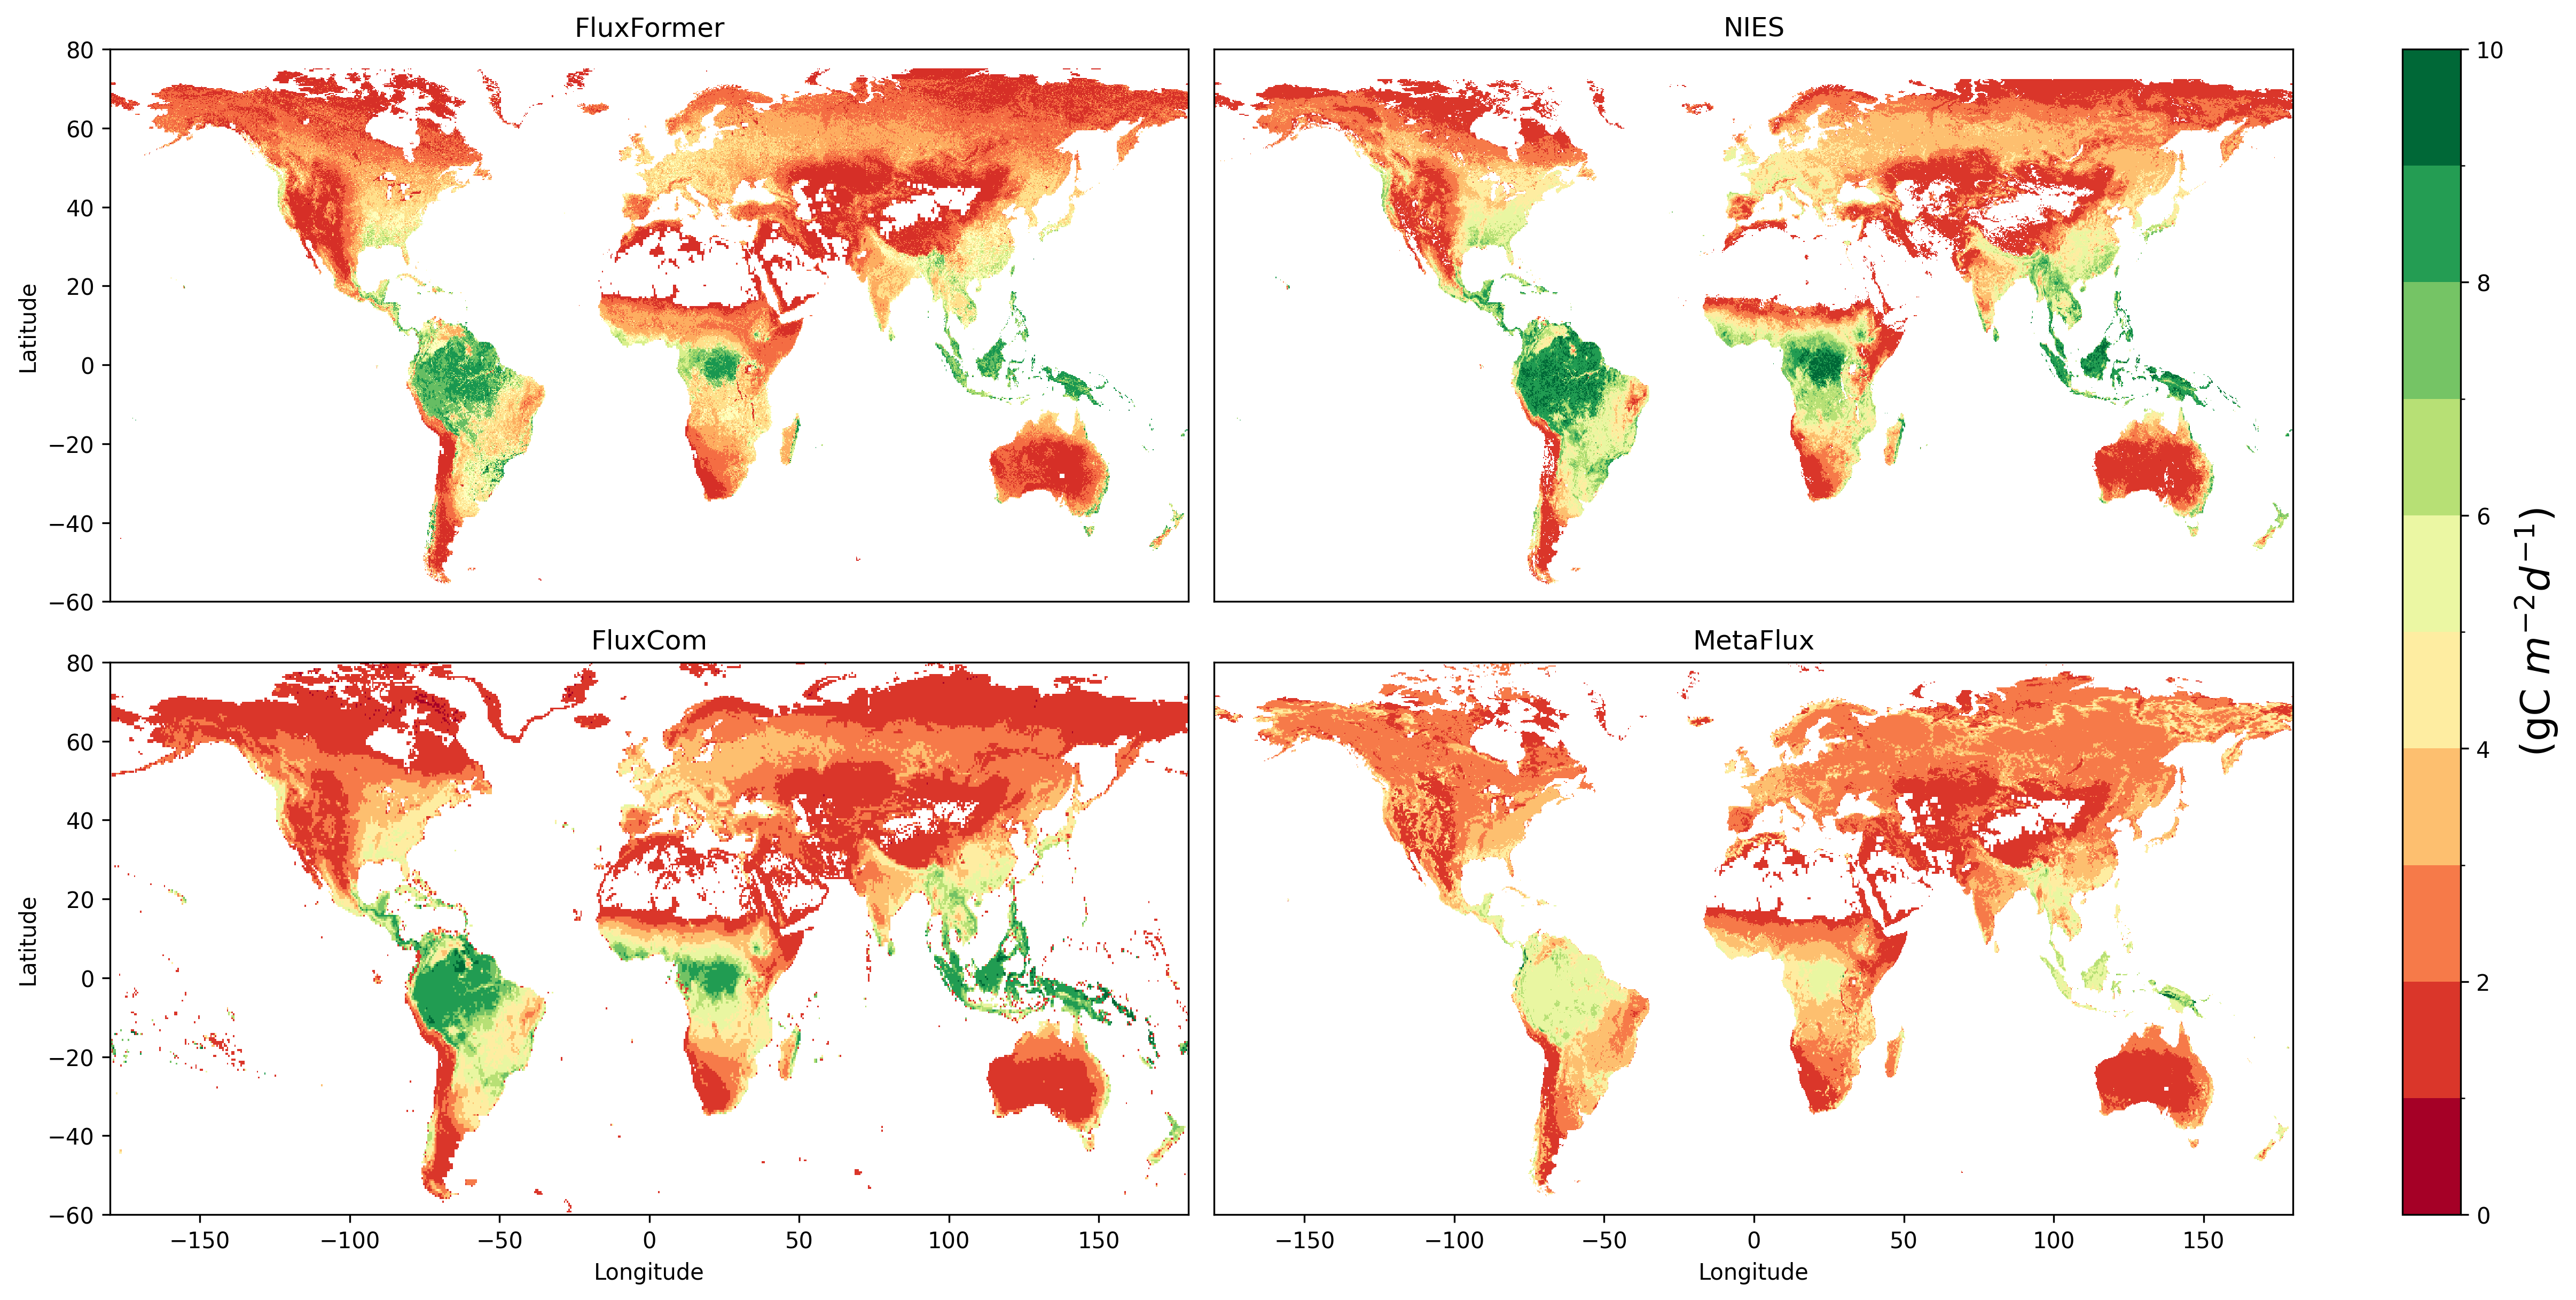
\includegraphics[width=\textwidth]{figs/chap6/GPP_2017_mean.png}
      \caption{GPP}
      \label{fig:chap6_fig2a}
    \end{subfigure}

    \begin{subfigure}{\textwidth}
      \centering
      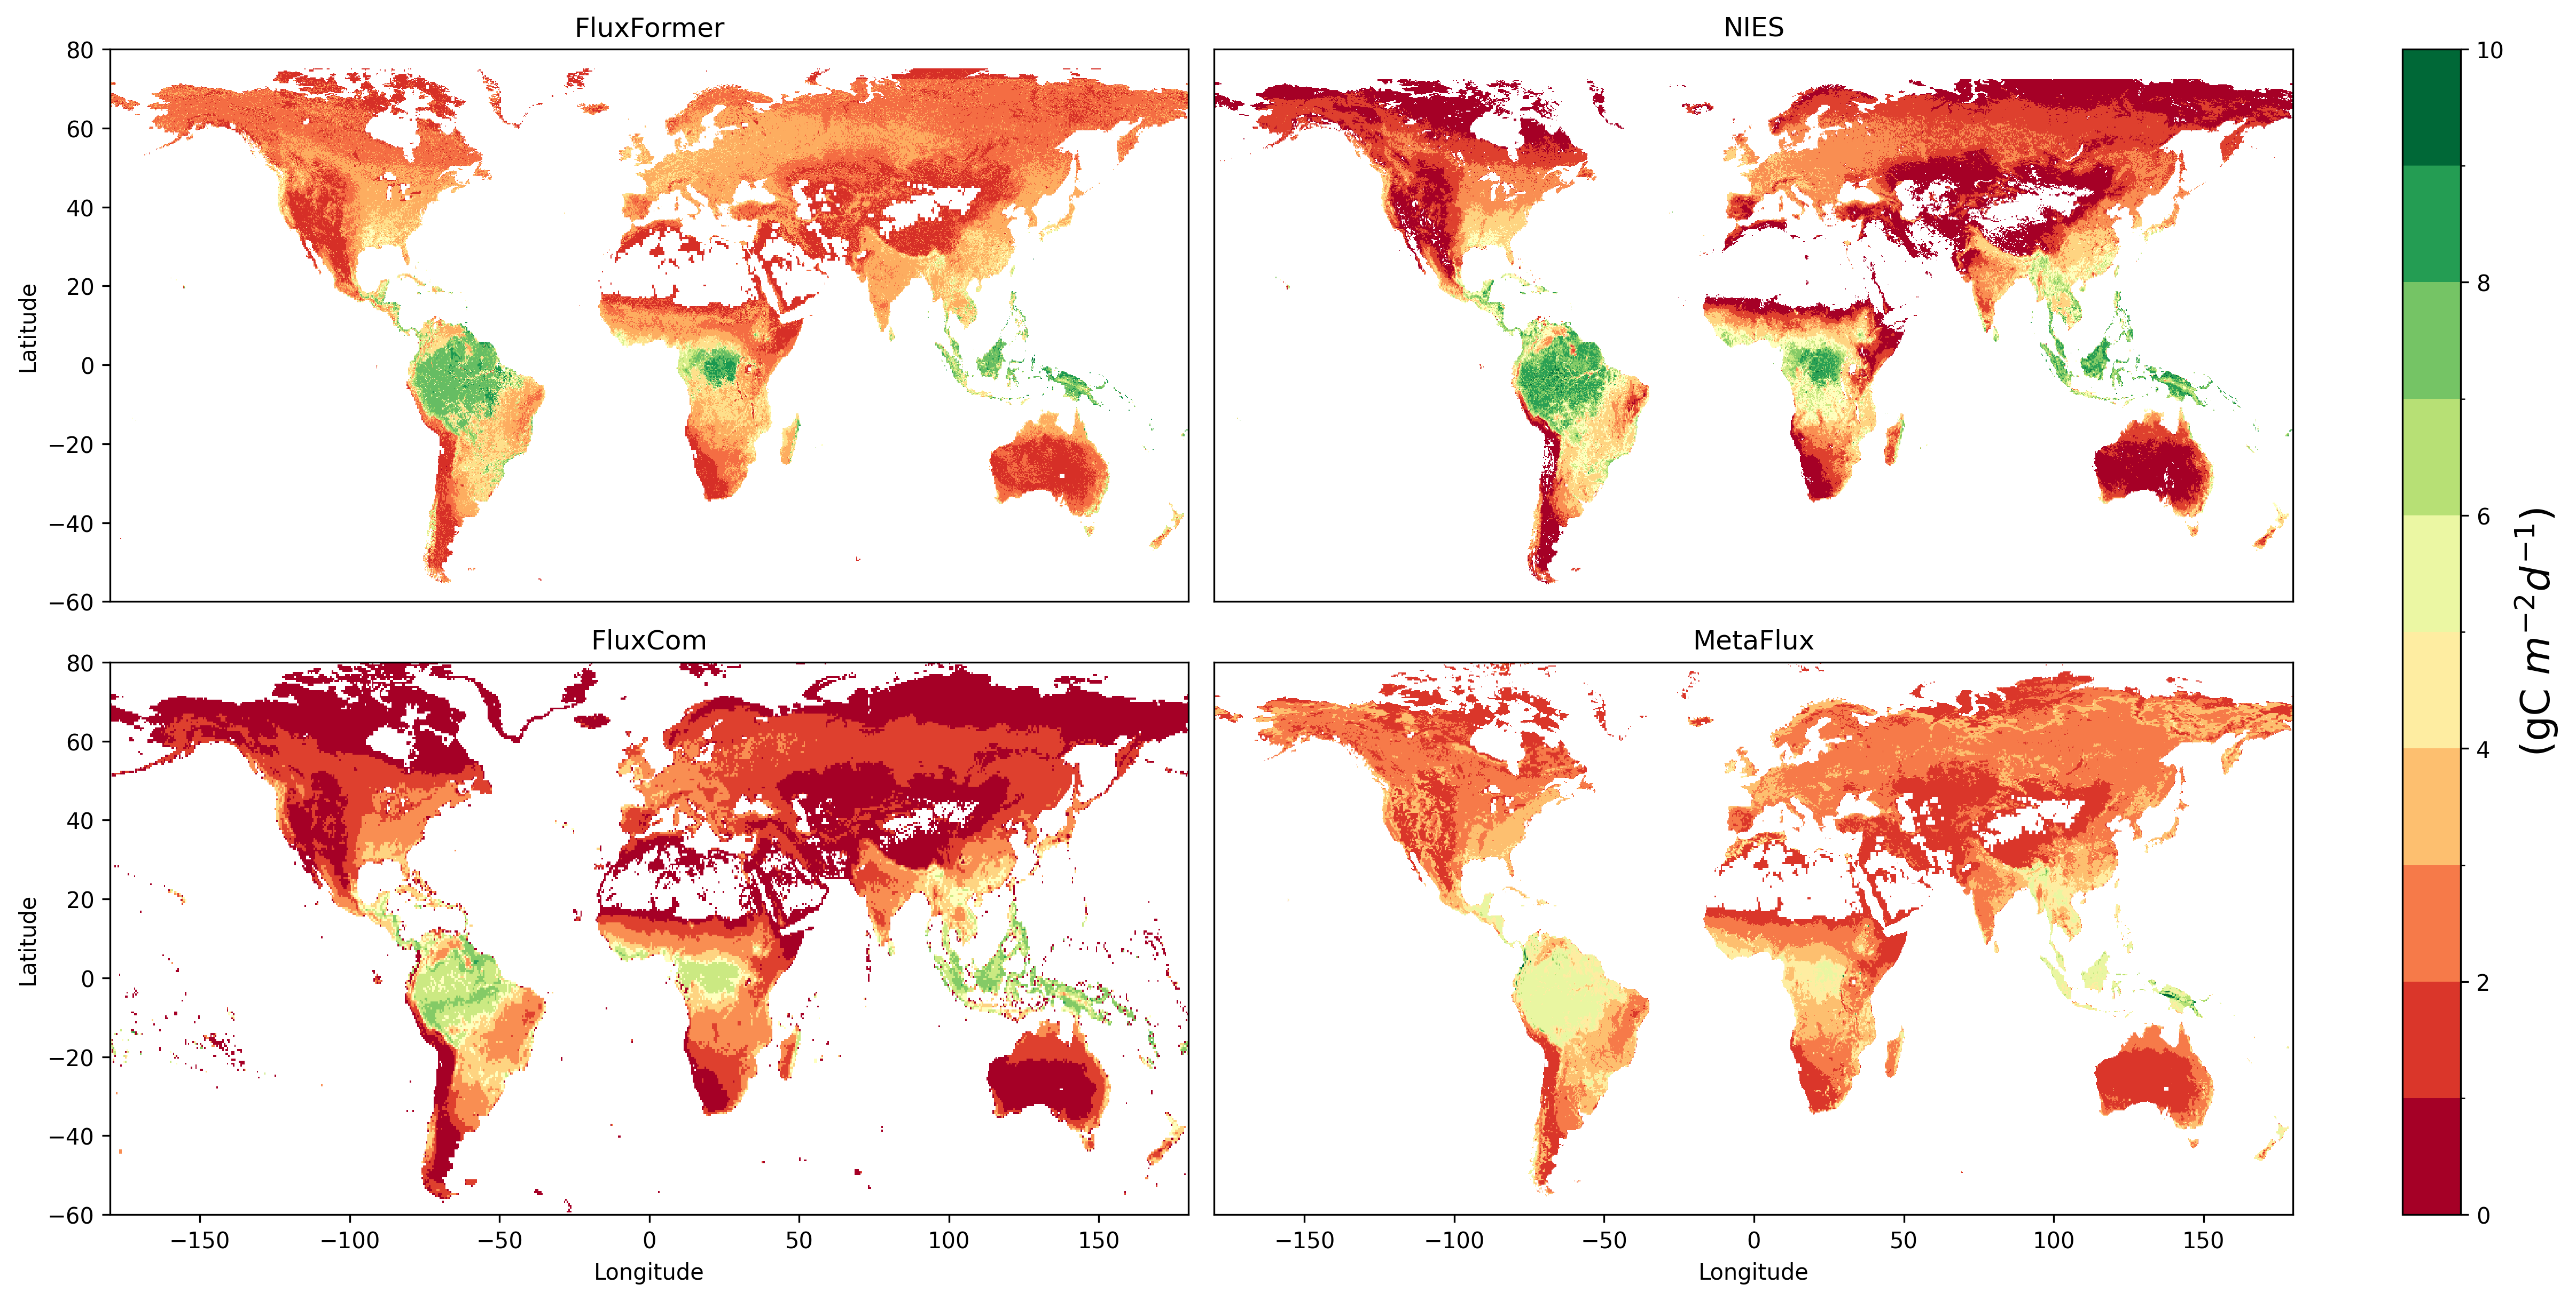
\includegraphics[width=\textwidth]{figs/chap6/RECO_2017_mean.png}
      \caption{RECO}
      \label{fig:chap6_fig2b}
    \end{subfigure}
    \caption[Mean estimate of GPP and RECO in 2017]{Mean estimate of (a) GPP and (b) RECO for the year 2017: GPP (a) RECO (b)}
    \label{fig:chap6_fig2}
\end{figure}
We show an example of our GPP in Figure \ref{fig:chap6_fig2a} and RECO in \ref{fig:chap6_fig2b} in comparison with other selected satellite-based upscaled products. We can observed that despite the uncertainties between the products, highest GPP and RECO values in tropical regions and lowest values in the semi-arid regions in all products. \par

\subsection{Technical validation}
\subsubsection*{Validation with FLUXNET 2015}
\paragraph*{Site-level validation}
We utilized the Pearson Correlation Coefficient (R) and Root Mean Square Error (RMSE) to assess the quality of our products in comparison to FLUXNET 2015 observations. As depicted in Figures \ref{fig:chap6_fig3a} and \ref{fig:chap6_fig3b}, our product demonstrates the highest correlation and the lowest RMSE with FLUXNET 2015 for both Gross Primary Productivity (GPP) and Ecosystem Respiration (RECO) data ($R = 0.894, RMSE = 1.706$ for GPP and $R = 0.866, RMSE = 1.244$ for RECO). In contrast, MetaFlux shows the lowest correlation with FLUXNET 2015 ($R = 0.652, RMSE = 3.135$ for GPP and $R = 0.612, RMSE = 2.046$ for RECO). NIES and FLUXCOM also exhibit strong correlations with the ground truth data, achieving $R/RMSE: 0.857/1.981$ (NIES), $0.819/2.32$ (FLUXCOM) for GPP and $R/RMSE: 0.795/1.511$ (NIES), $0.792/1.627$ (FLUXCOM) for RECO. \par

\begin{figure}[p]
    \centering
    \begin{subfigure}{\textwidth}
      \centering
      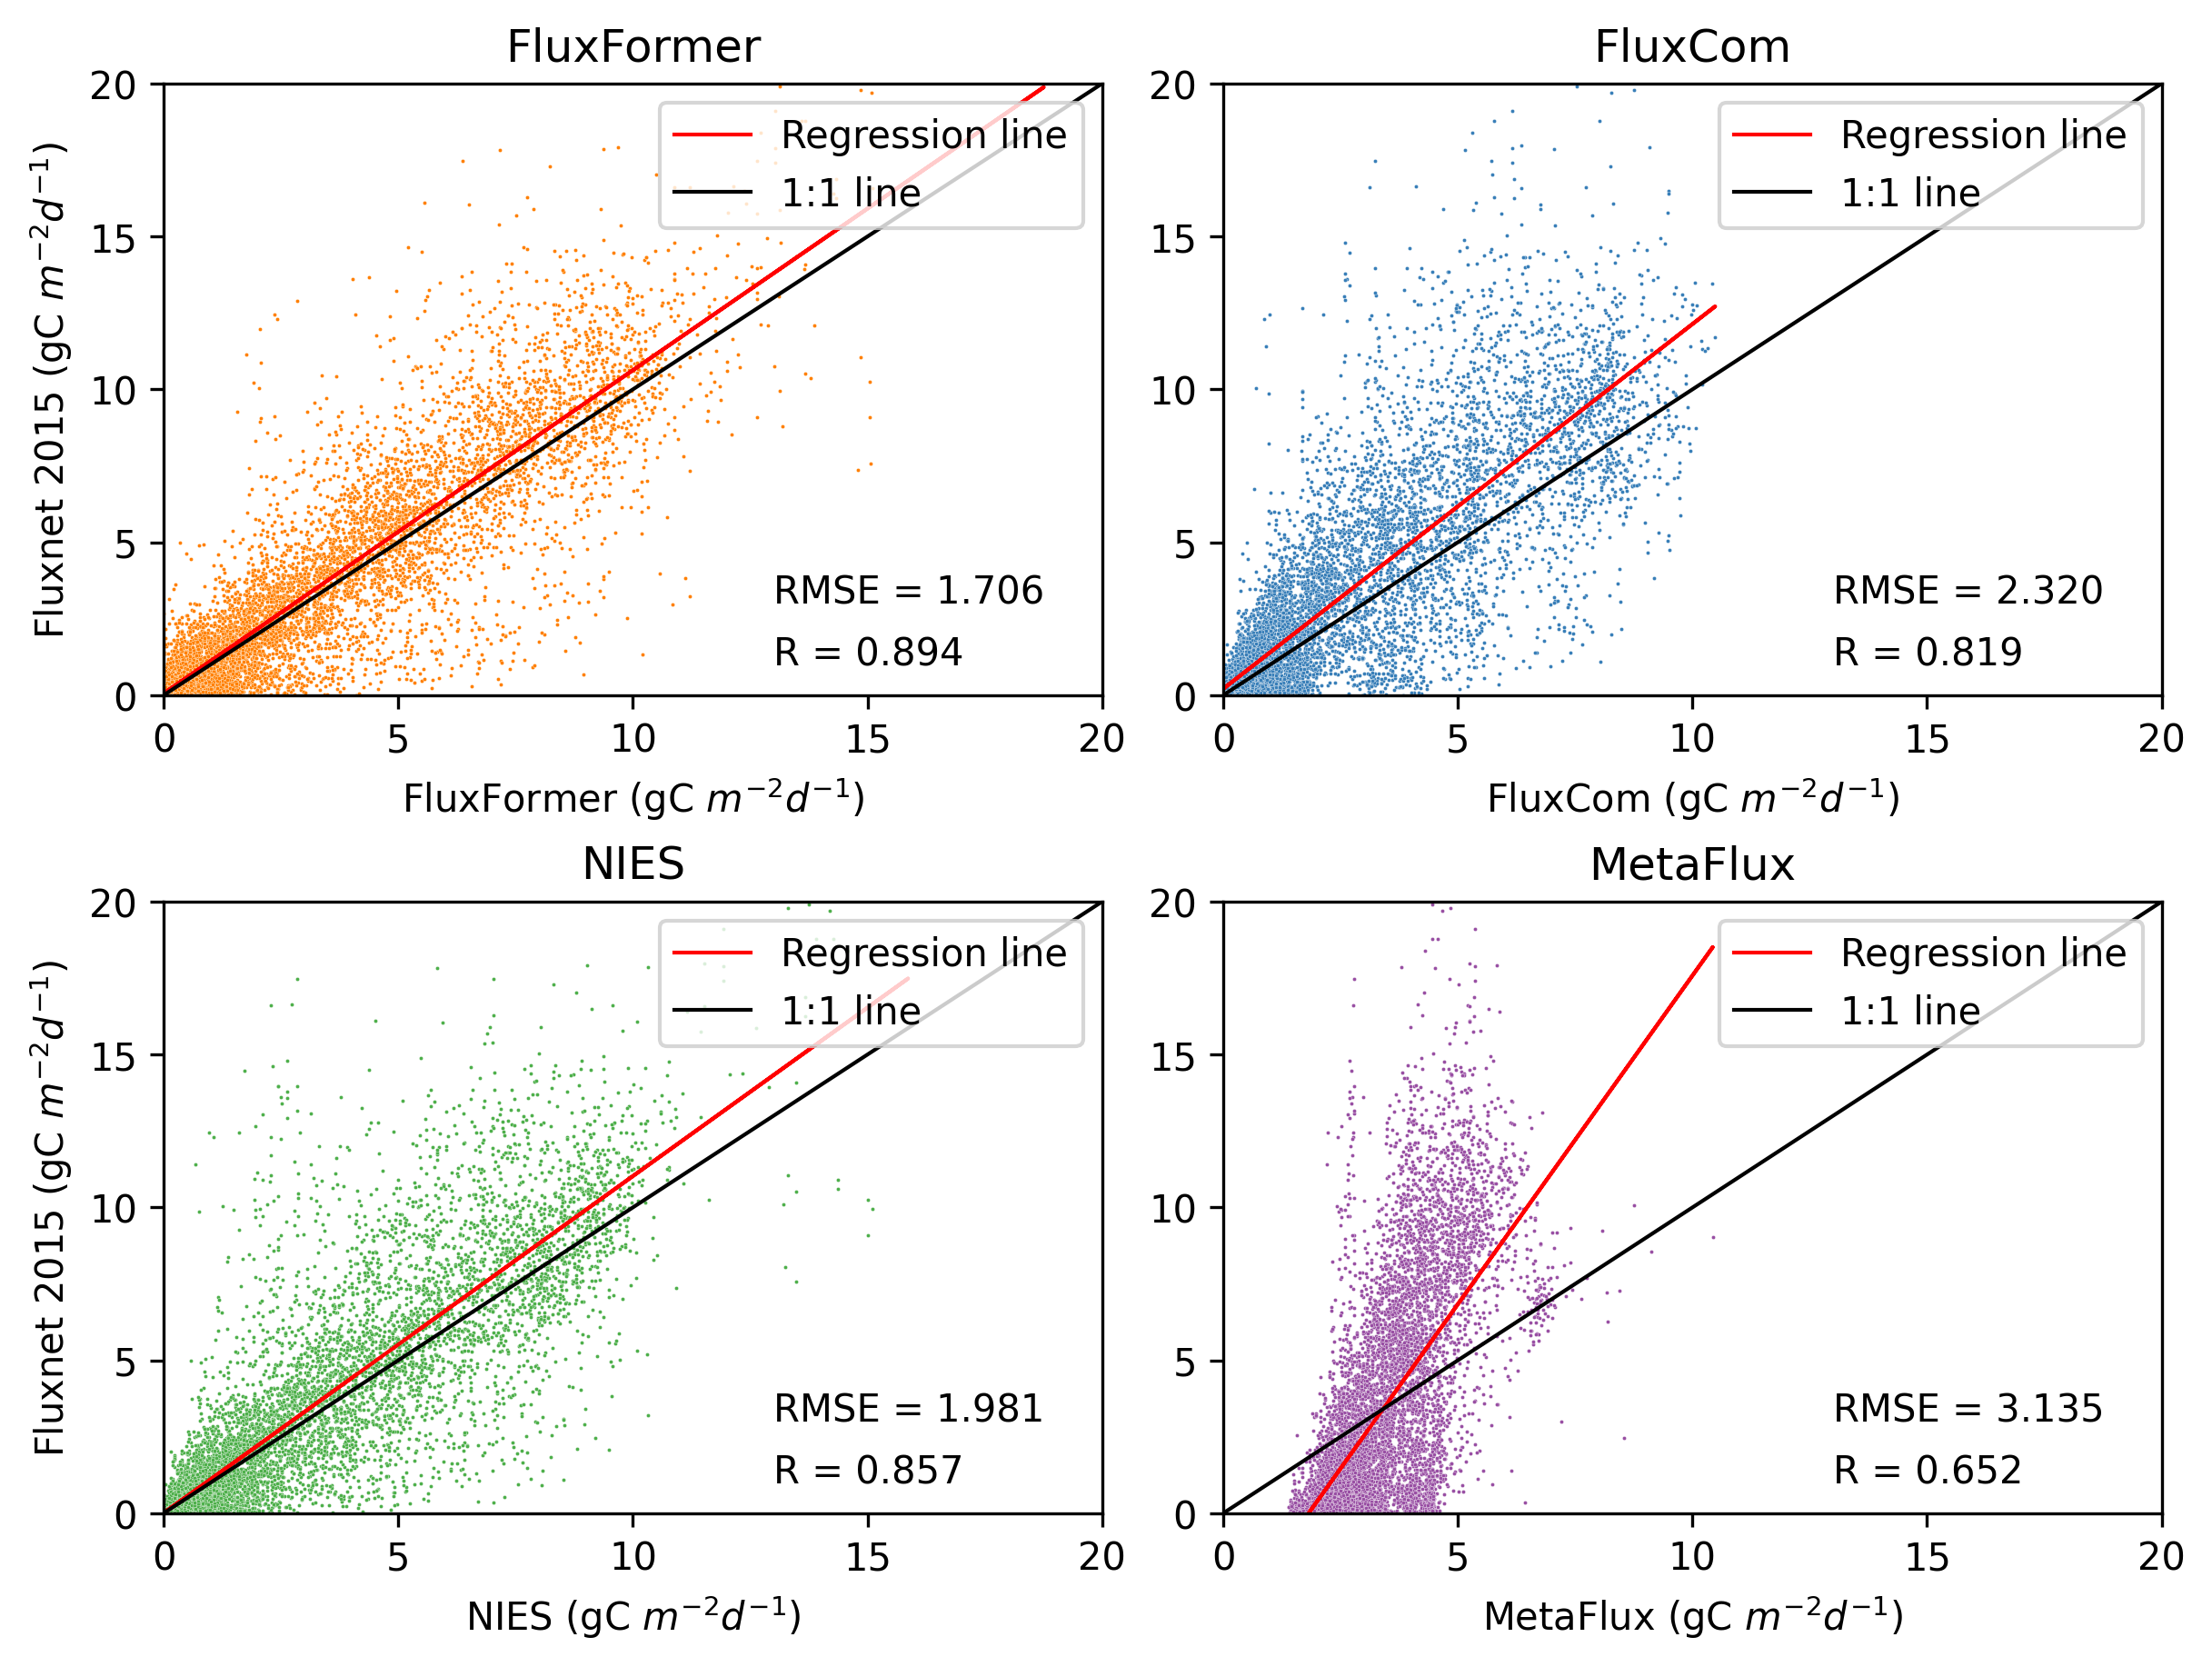
\includegraphics[width=.8\textwidth]{figs/chap6/val_fluxnet_all_GPP.png}
      \caption{GPP}
      \label{fig:chap6_fig3a}
    \end{subfigure}

    \begin{subfigure}{\textwidth}
      \centering
      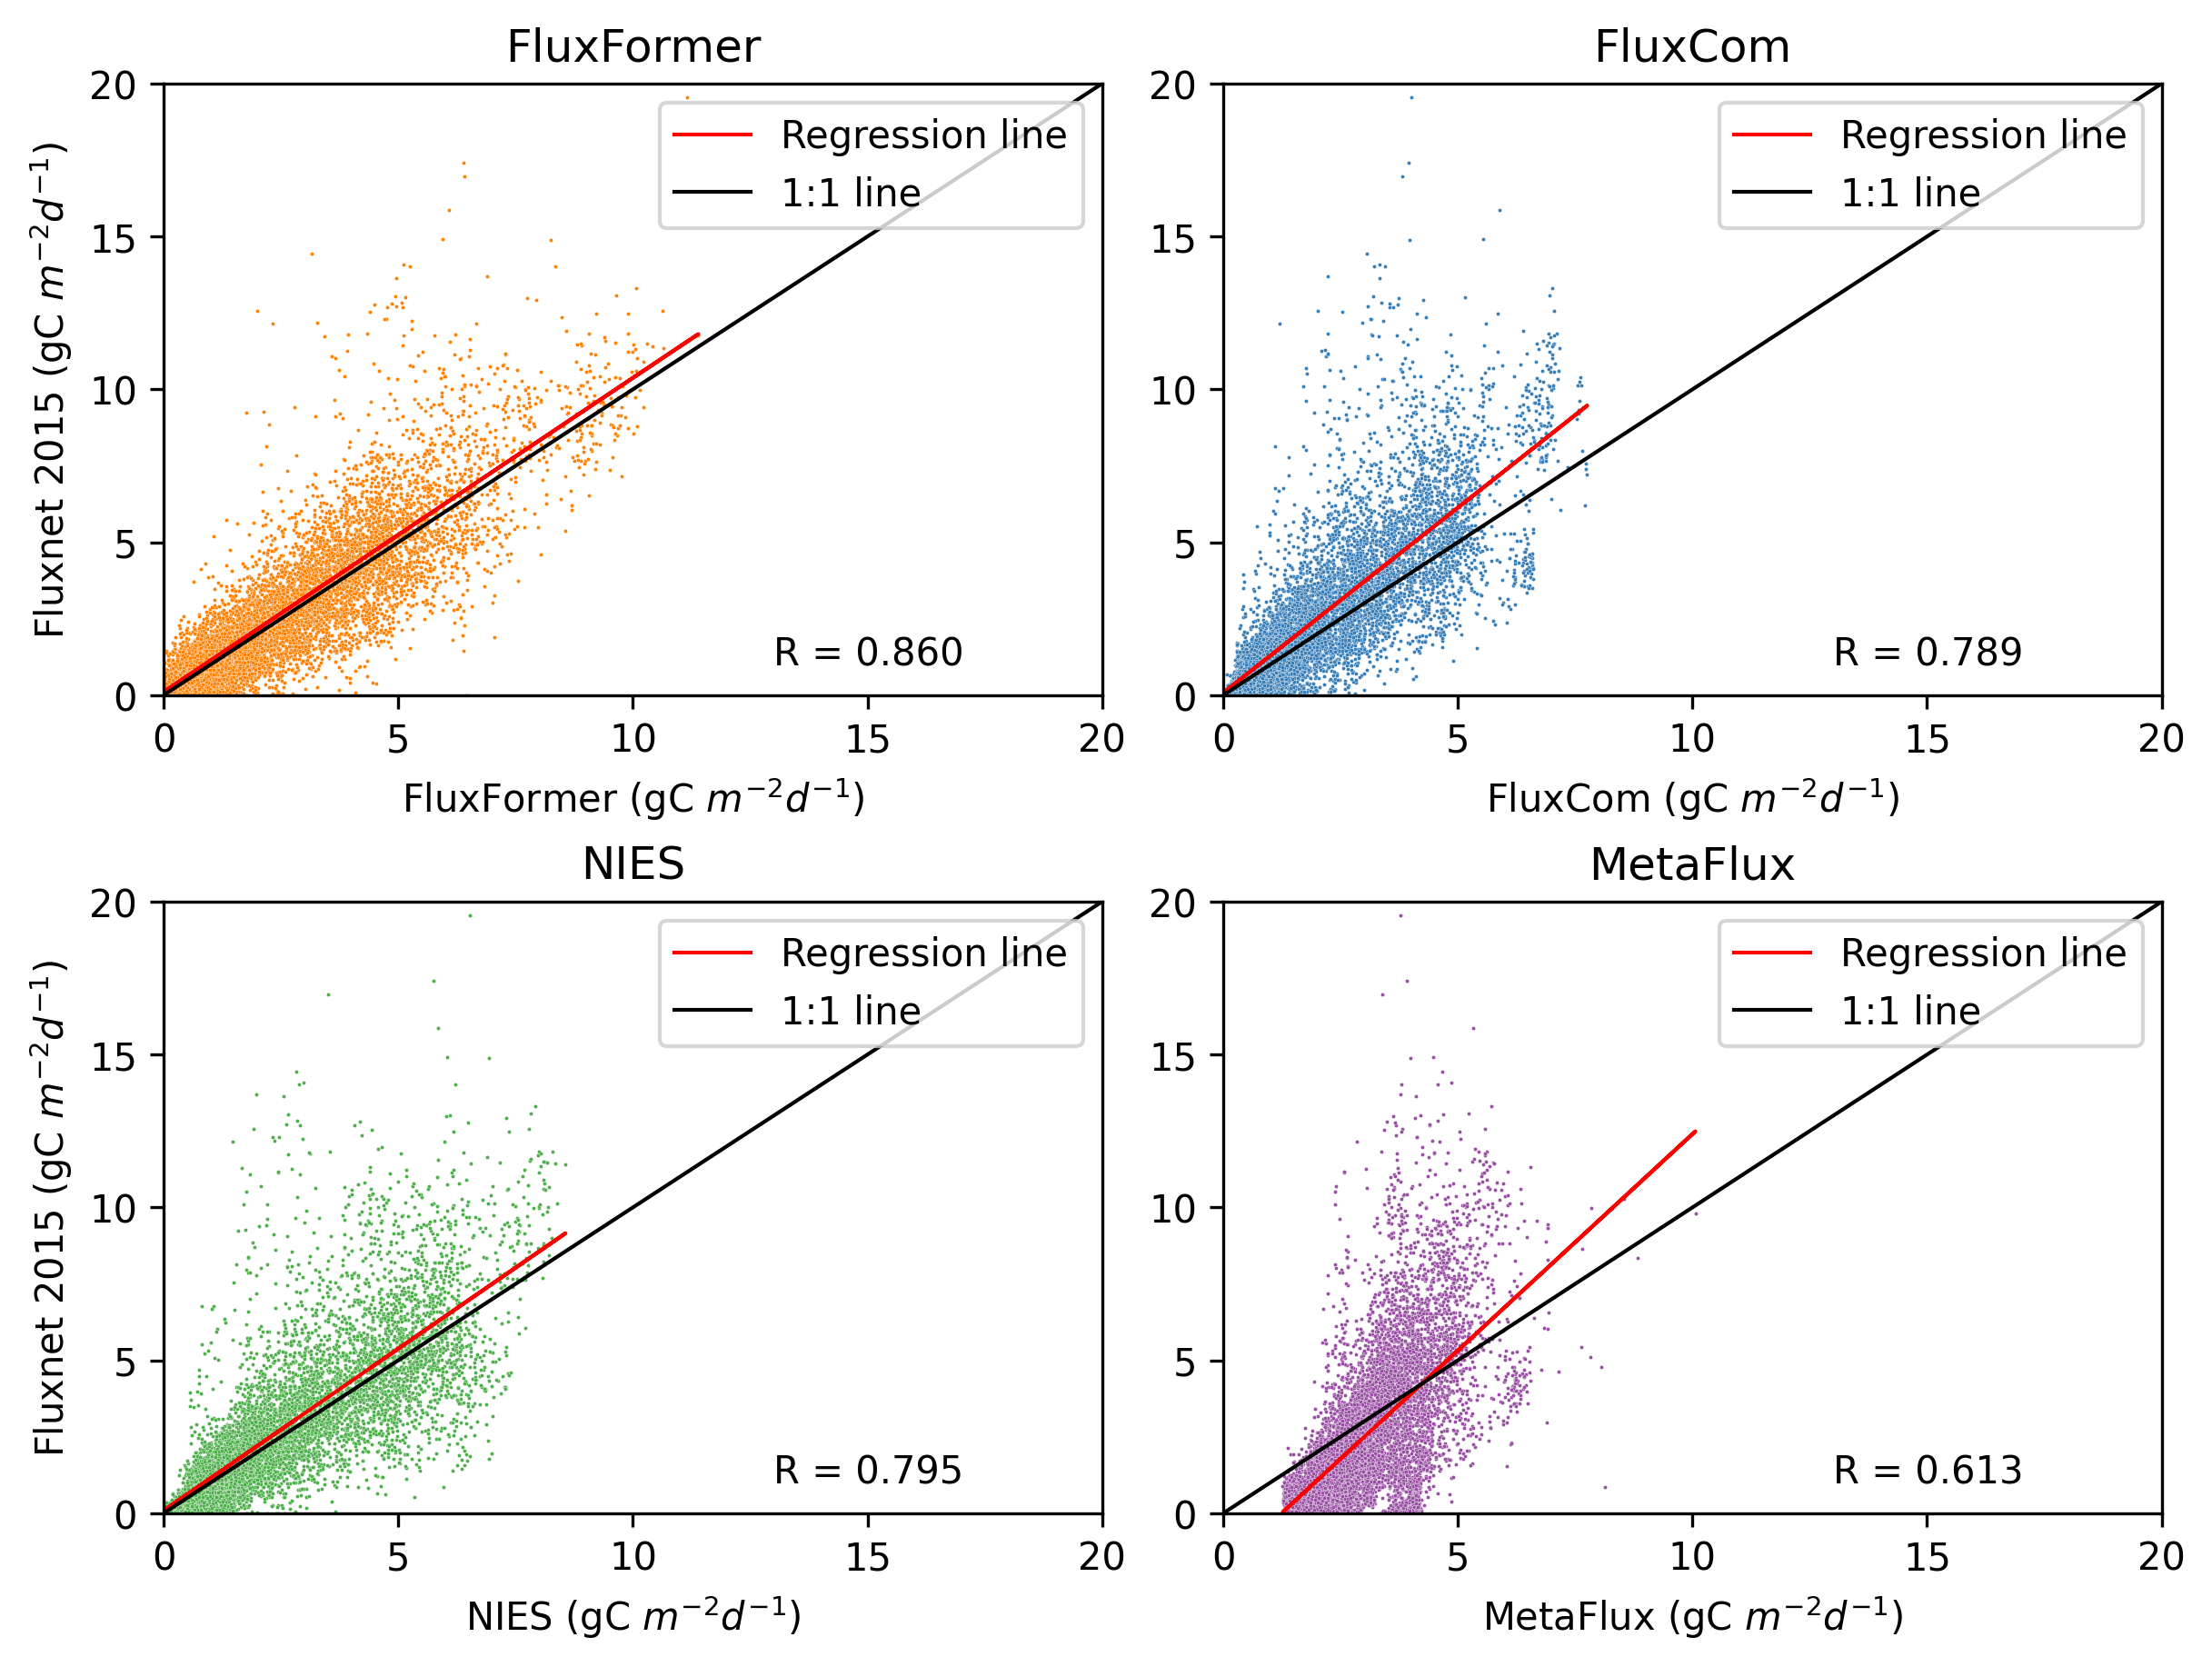
\includegraphics[width=.8\textwidth]{figs/chap6/val_fluxnet_all_RECO.png}
      \caption{RECO}
      \label{fig:chap6_fig3b}
    \end{subfigure}
    \caption[Validation with FLUXNET 2015]{Validation with FLUXNET 2015: GPP (a) RECO (b)}
    \label{fig:chap6_fig3}
\end{figure}
\paragraph*{Seasonality validation}
We analyzed the seasonal trend using FLUXNET 2015 data, calculating monthly mean values across climate zones, as depicted in Figure \ref{fig:chap6_fig4} and Table \ref{tab}. In arid regions, FluxFormer, FluxCom, and NIES exhibited high correlation ($R > 0.9$) with FLUXNET for both GPP and RECO. However, MetaFlux showed lower correlation with $R=0.48$ for GPP and $R=0.66$ for RECO in arid regions. For temperate and cold regions, all satellite-based products (FluxFormer, FLUXCOM, NIES, and MetaFlux) demonstrated high correlations ($R>0.97$) with FLUXNET 2015 GPP and RECO. \par

\begin{table}[!ht]
    \centering
    \caption{Pearson correlation of seasonal trend with FLUXNET 2015}
    \begin{tabular}{ccccc}
        \hline
        Climate groups & FluxFormer & FluxCom & NIES & MetaFlux  \\ \hline
        \multicolumn{5}{c}{GPP}   \\ \hline 
        Arid & 0.91 & 0.91 & 0.94 & 0.48  \\ \hline 
        Temperate & 0.99 & 0.99 & 0.97 & 0.97  \\ \hline 
        Cold & 1 & 0.99 & 1 & 0.99  \\ \hline 
        Trop. SVN & 0.99 & 0.99 & 0.94 & 0.97  \\ \hline 
        Trop. MS & \textbf{0.84} & 0.04 & 0.58 & -0.05  \\ \hline 
        Trop. RF & 0.68 & 0.6 & 0.71 & 0.41  \\ \hline 
        \multicolumn{5}{c}{RECO}   \\ \hline 
        Arid & 0.94 & 0.92 & 0.95 & 0.66  \\ \hline 
        Temperate & 0.98 & 0.99 & 0.99 & 0.99  \\ \hline 
        Cold & 1 & 0.99 & 1 & 1  \\ \hline 
        Trop. SVN & 0.99 & 0.98 & 0.92 & 0.91  \\ \hline 
        Trop. MS & \textbf{0.88} & 0.51 & 0.29 & 0  \\ \hline 
        Trop. RF & \textbf{0.68} & 0.37 & 0.5 & 0.47  \\ \hline 
    \end{tabular}
    \label{tab:chap6_seasonr}
\end{table}
\begin{figure}[p]
    \centering
    \begin{subfigure}{\textwidth}
      \centering
      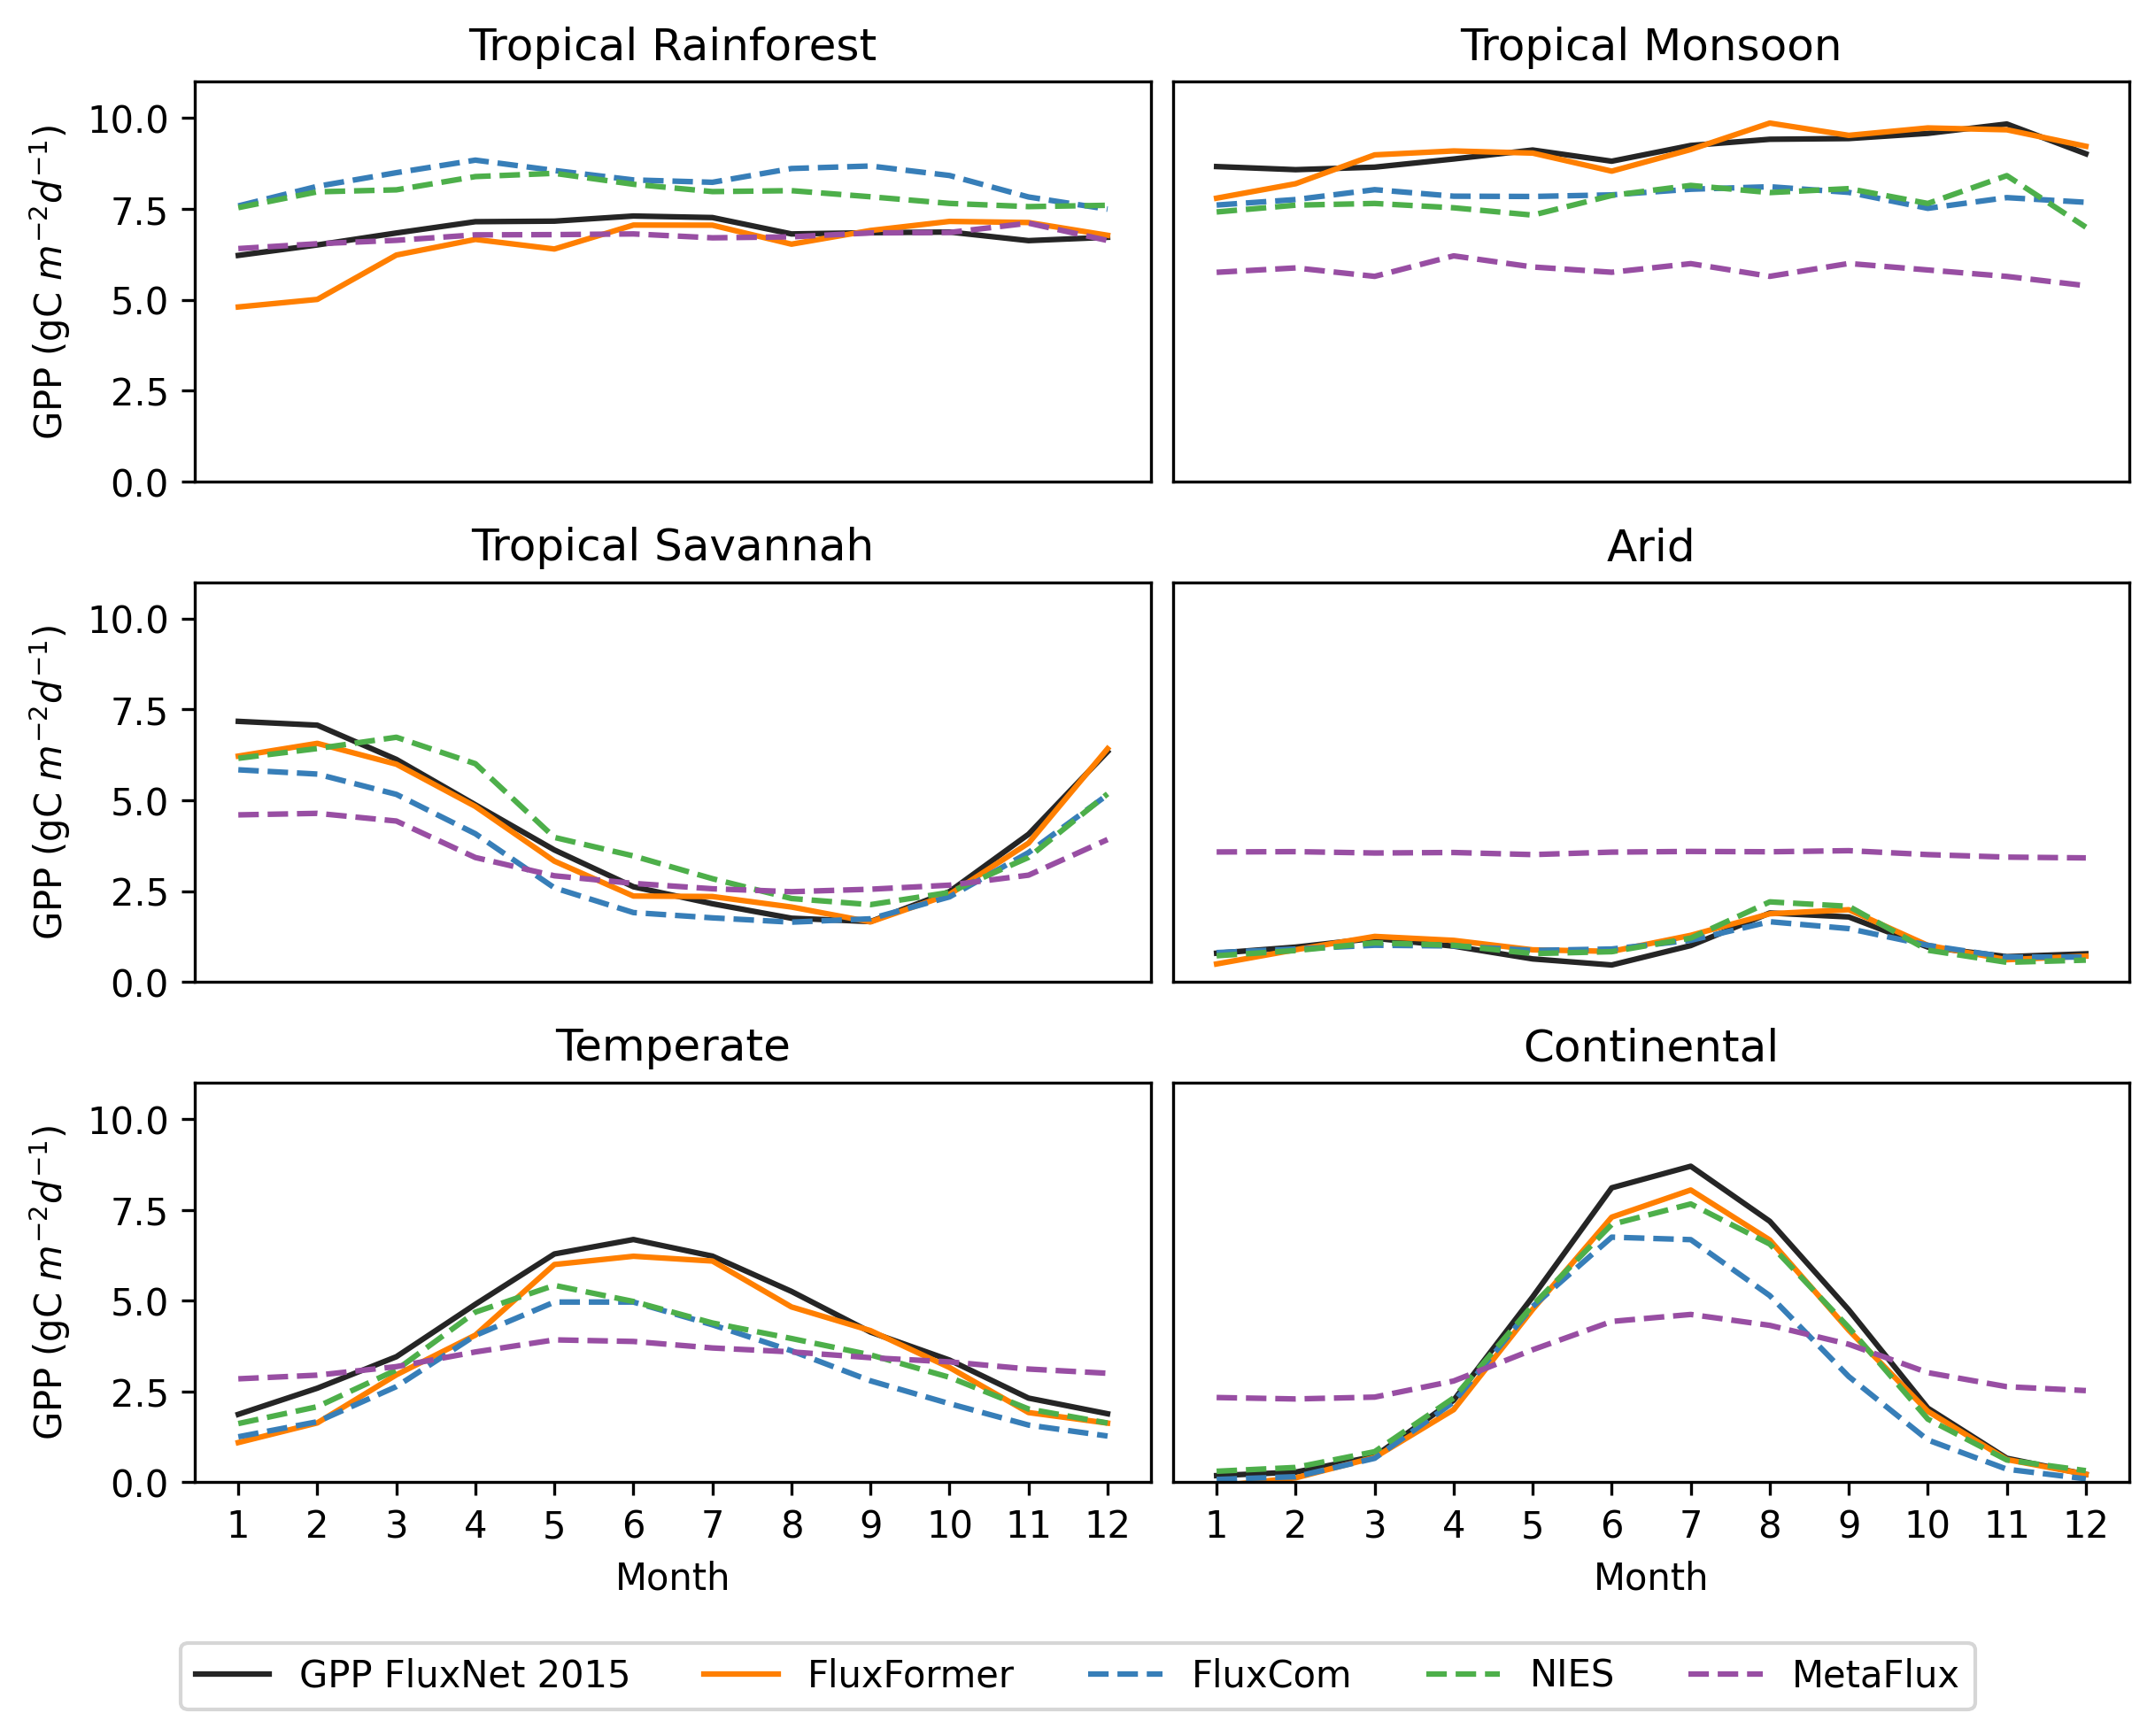
\includegraphics[width=.8\textwidth]{figs/chap6/seasonal_fluxnet_GPP.png}
      \caption{GPP}
      \label{fig:chap6_fig4a}
    \end{subfigure}

    \begin{subfigure}{\textwidth}
      \centering
      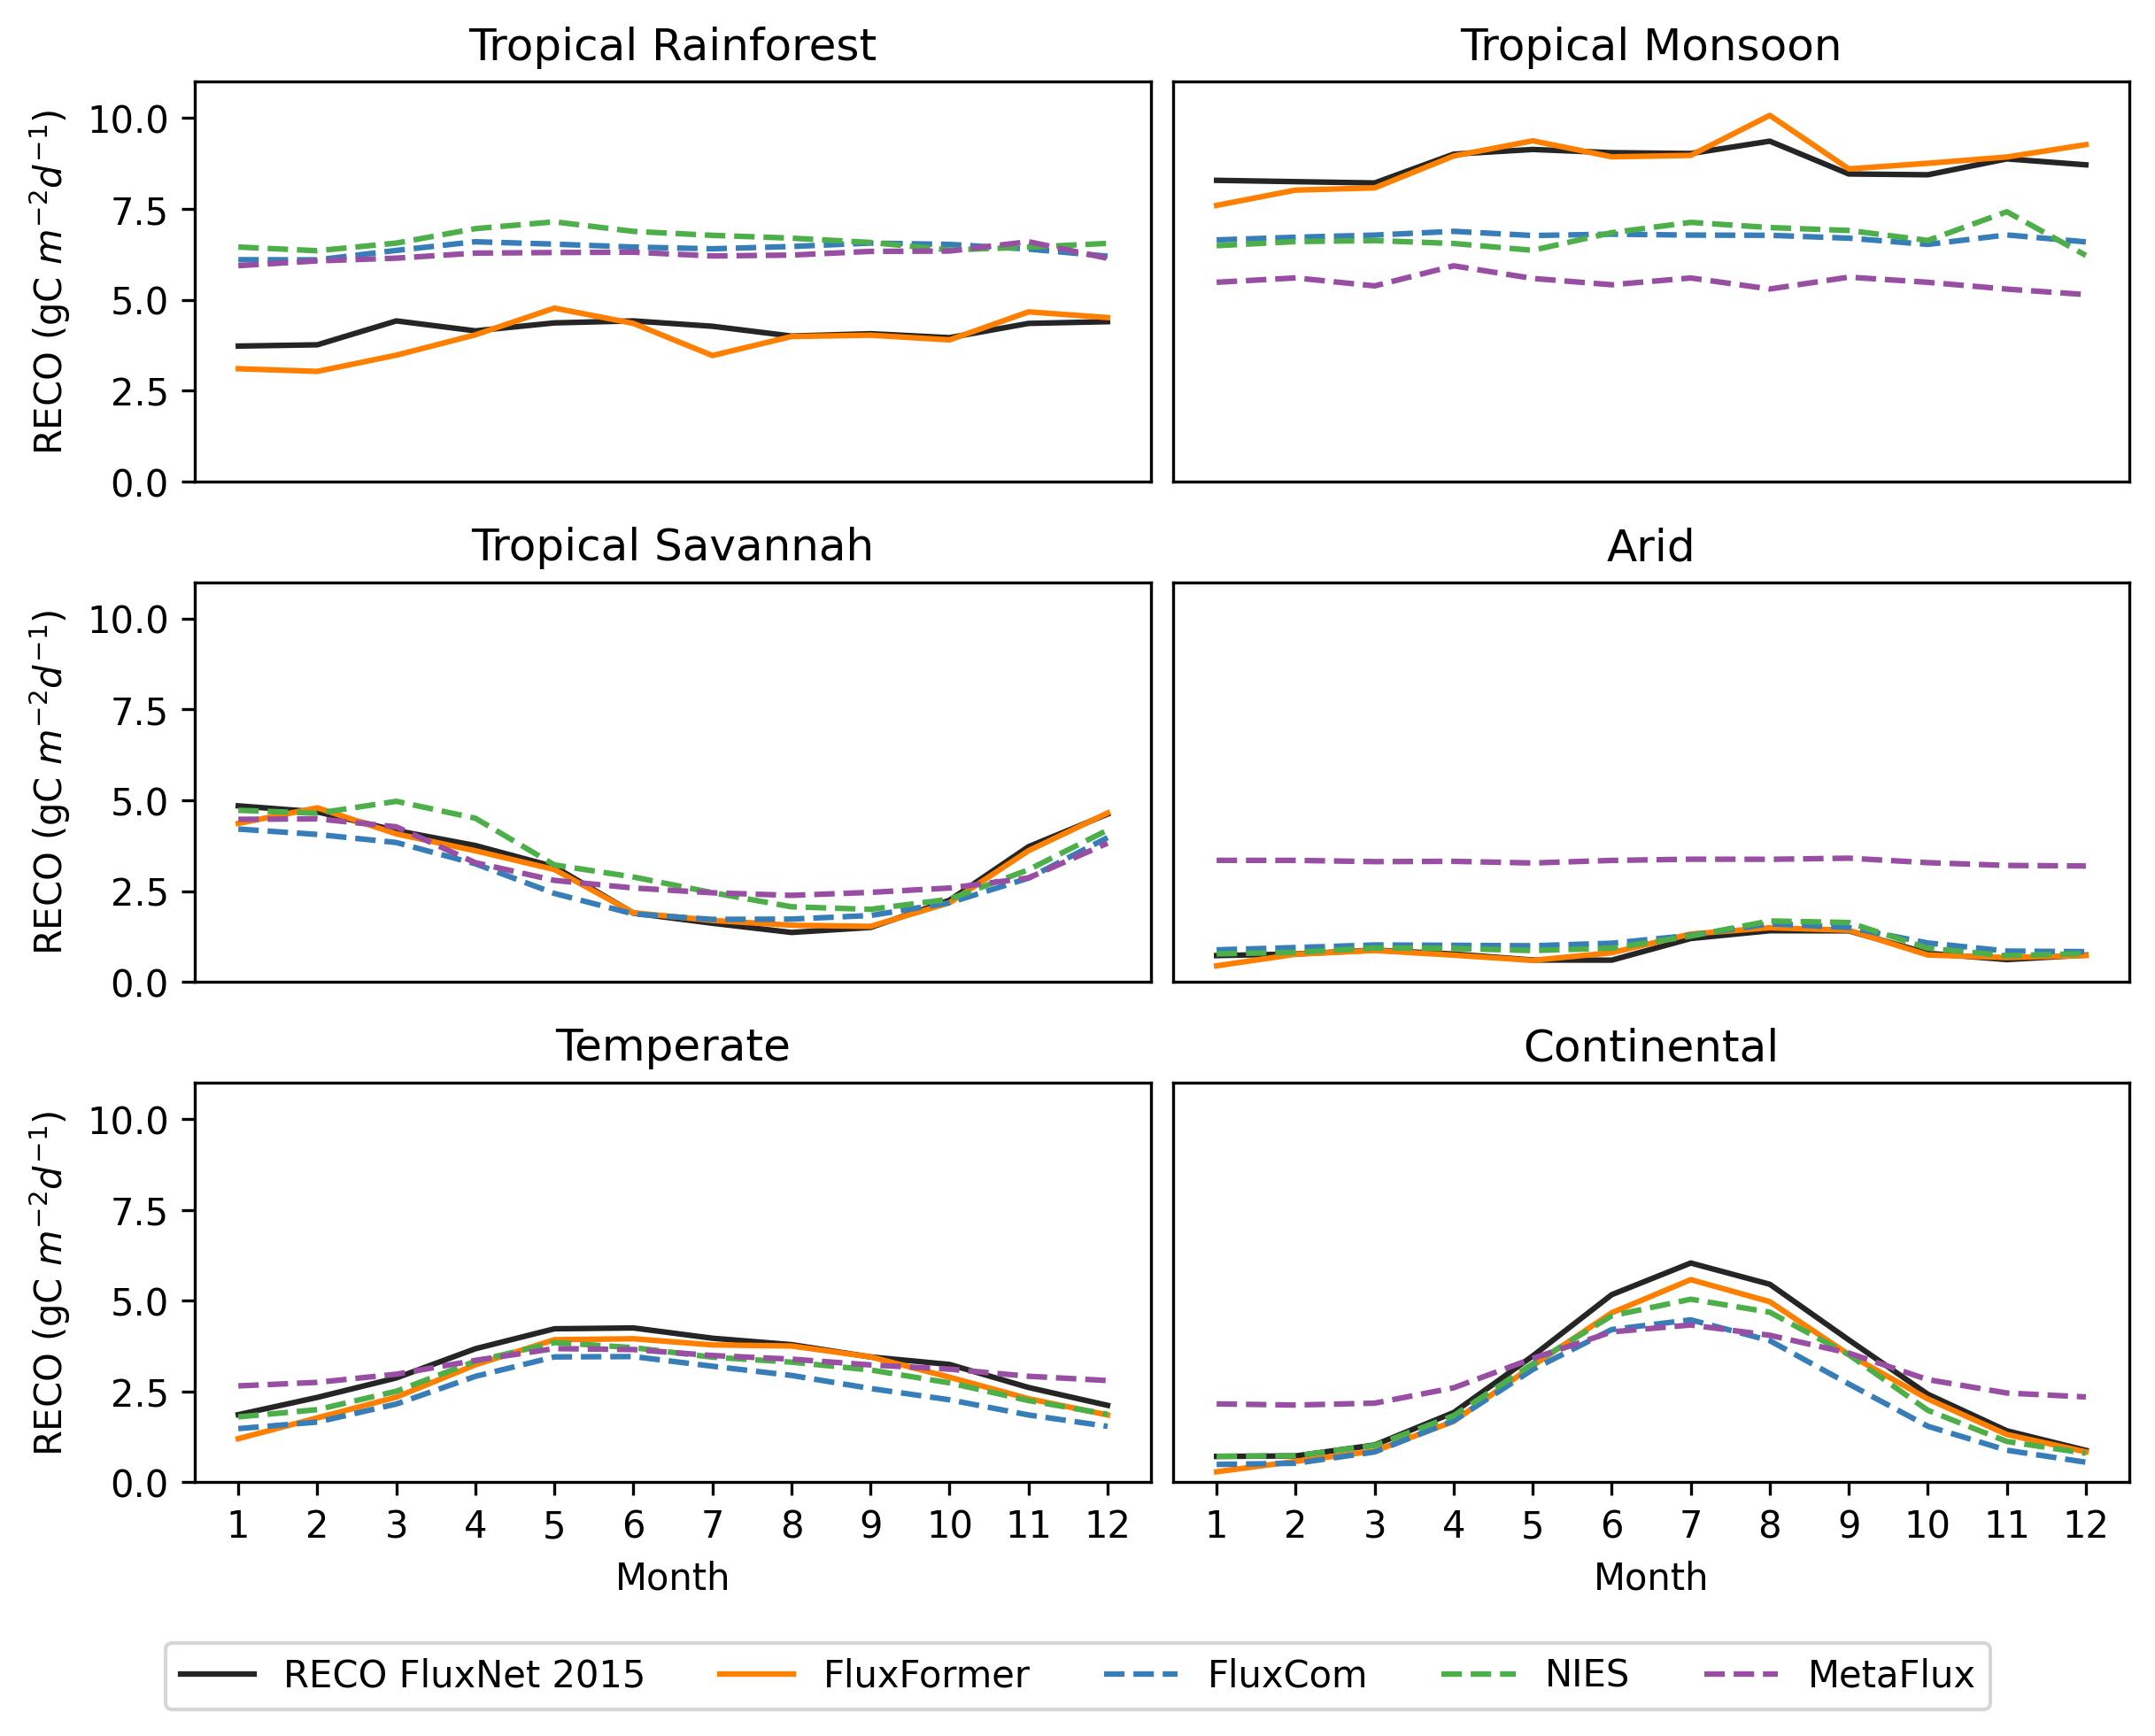
\includegraphics[width=.8\textwidth]{figs/chap6/seasonal_fluxnet_RECO.png}
      \caption{RECO}
      \label{fig:chap6_fig4b}
    \end{subfigure}
    \caption[Seasonality validation with FLUXNET 2015]{Seasonality validation with FLUXNET 2015: GPP (a) RECO (b)}
    \label{fig:chap6_fig4}
\end{figure}
In the tropical region, we partitioned the area into tropical savanna (Trop. SVN), tropical monsoon (Trop. MS), and tropical rainforest (Trop. RF). In Trop. SVN, all satellite-based products displayed a high correlation with FLUXNET 2015 for both GPP and RECO. Conversely, for Trop. MS, our data exhibited the highest correlation at $R=0.84$, while NIES data showed a moderate correlation ($R=0.58$). FLUXCOM and MetaFlux demonstrated no correlation with FLUXNET 2015 for GPP, with $R<0.1$. Regarding RECO in Trop. SVN, our data maintained the highest correlation with the seasonal trend of the ground truth, whereas other products showed lower correlation (FLUXCOM: $R=0.51$, NIES: $R=0.29$) or no correlation with the ground truth (MetaFlux: $R=0$). In the Trop. RF area, our data exhibited the second-highest correlation with GPP seasonal trend ($R=0.68$) and the highest correlation with RECO seasonal trend ($R=0.68$).\par
Overall, our data demonstrates a robust correlation in arid, temperate, cold, and Trop. SVN regions, surpassing $R> 0.9$ for both GPP and RECO. Specifically, in Trop. MS, our data exhibits the highest correlation, reaching $R=0.84$ for GPP and $R=0.88$ for RECO. In the Trop. RF region, our data exhibits the second-highest correlation with the ground truth GPP seasonal trend ($R=0.68$) and the highest correlation with the ground truth RECO seasonal trend ($R=0.68$) among the selected satellite-based products. \par


\subsubsection*{Validation with SIF}
SIF serves as a reliable proxy and has seen increased usage for estimating GPP \citep{norton2019estimating, liu2020improving, bai2022estimation}. To expand the seasonality validation, we incorporated independent products, namely CSIF and TROPOMI SIF. We examined the pixel-level correlation distribution of FluxFormer and selected satellite-based products with the seasonal trend of CSIF from 2000 to 2019 and TROPOMI SIF from 2018 to 2019, as TROPOMI data is available only from 2018 onwards.\par

\begin{figure}[tbh!]
    \centering
    \begin{subfigure}{\textwidth}
      \centering
      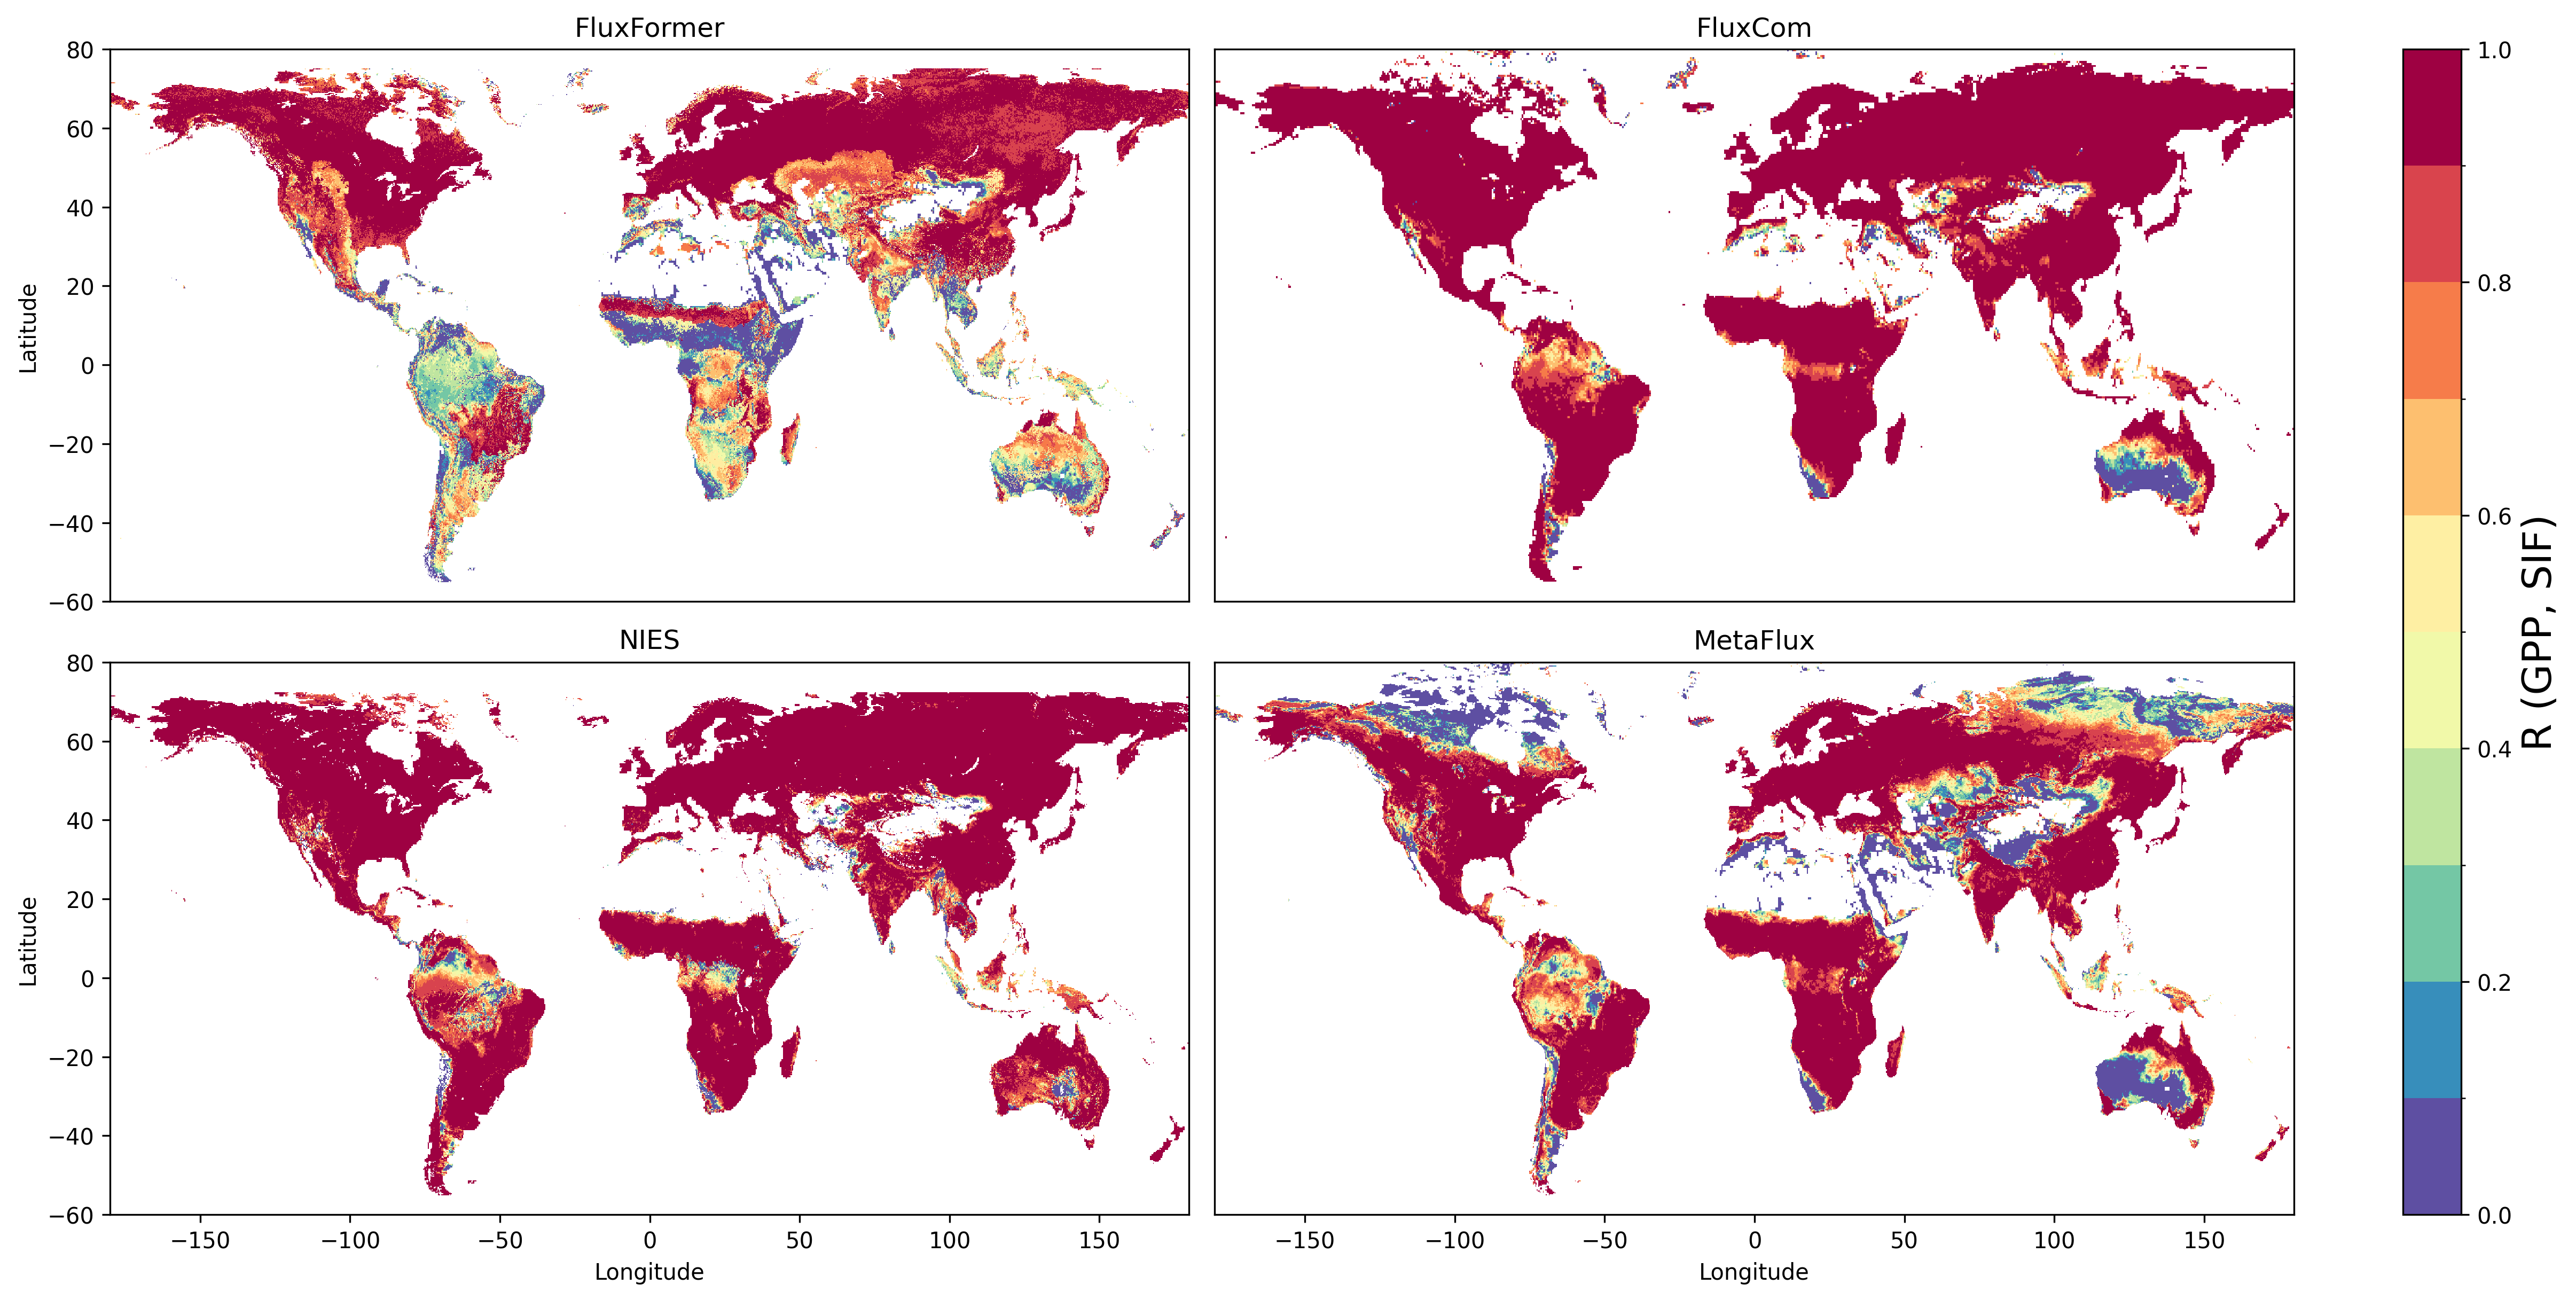
\includegraphics[width=\textwidth]{figs/chap6/val_CSIF.png}
      \caption{CSIF}
      \label{fig:chap6_fig5a}
    \end{subfigure}

    \begin{subfigure}{\textwidth}
      \centering
      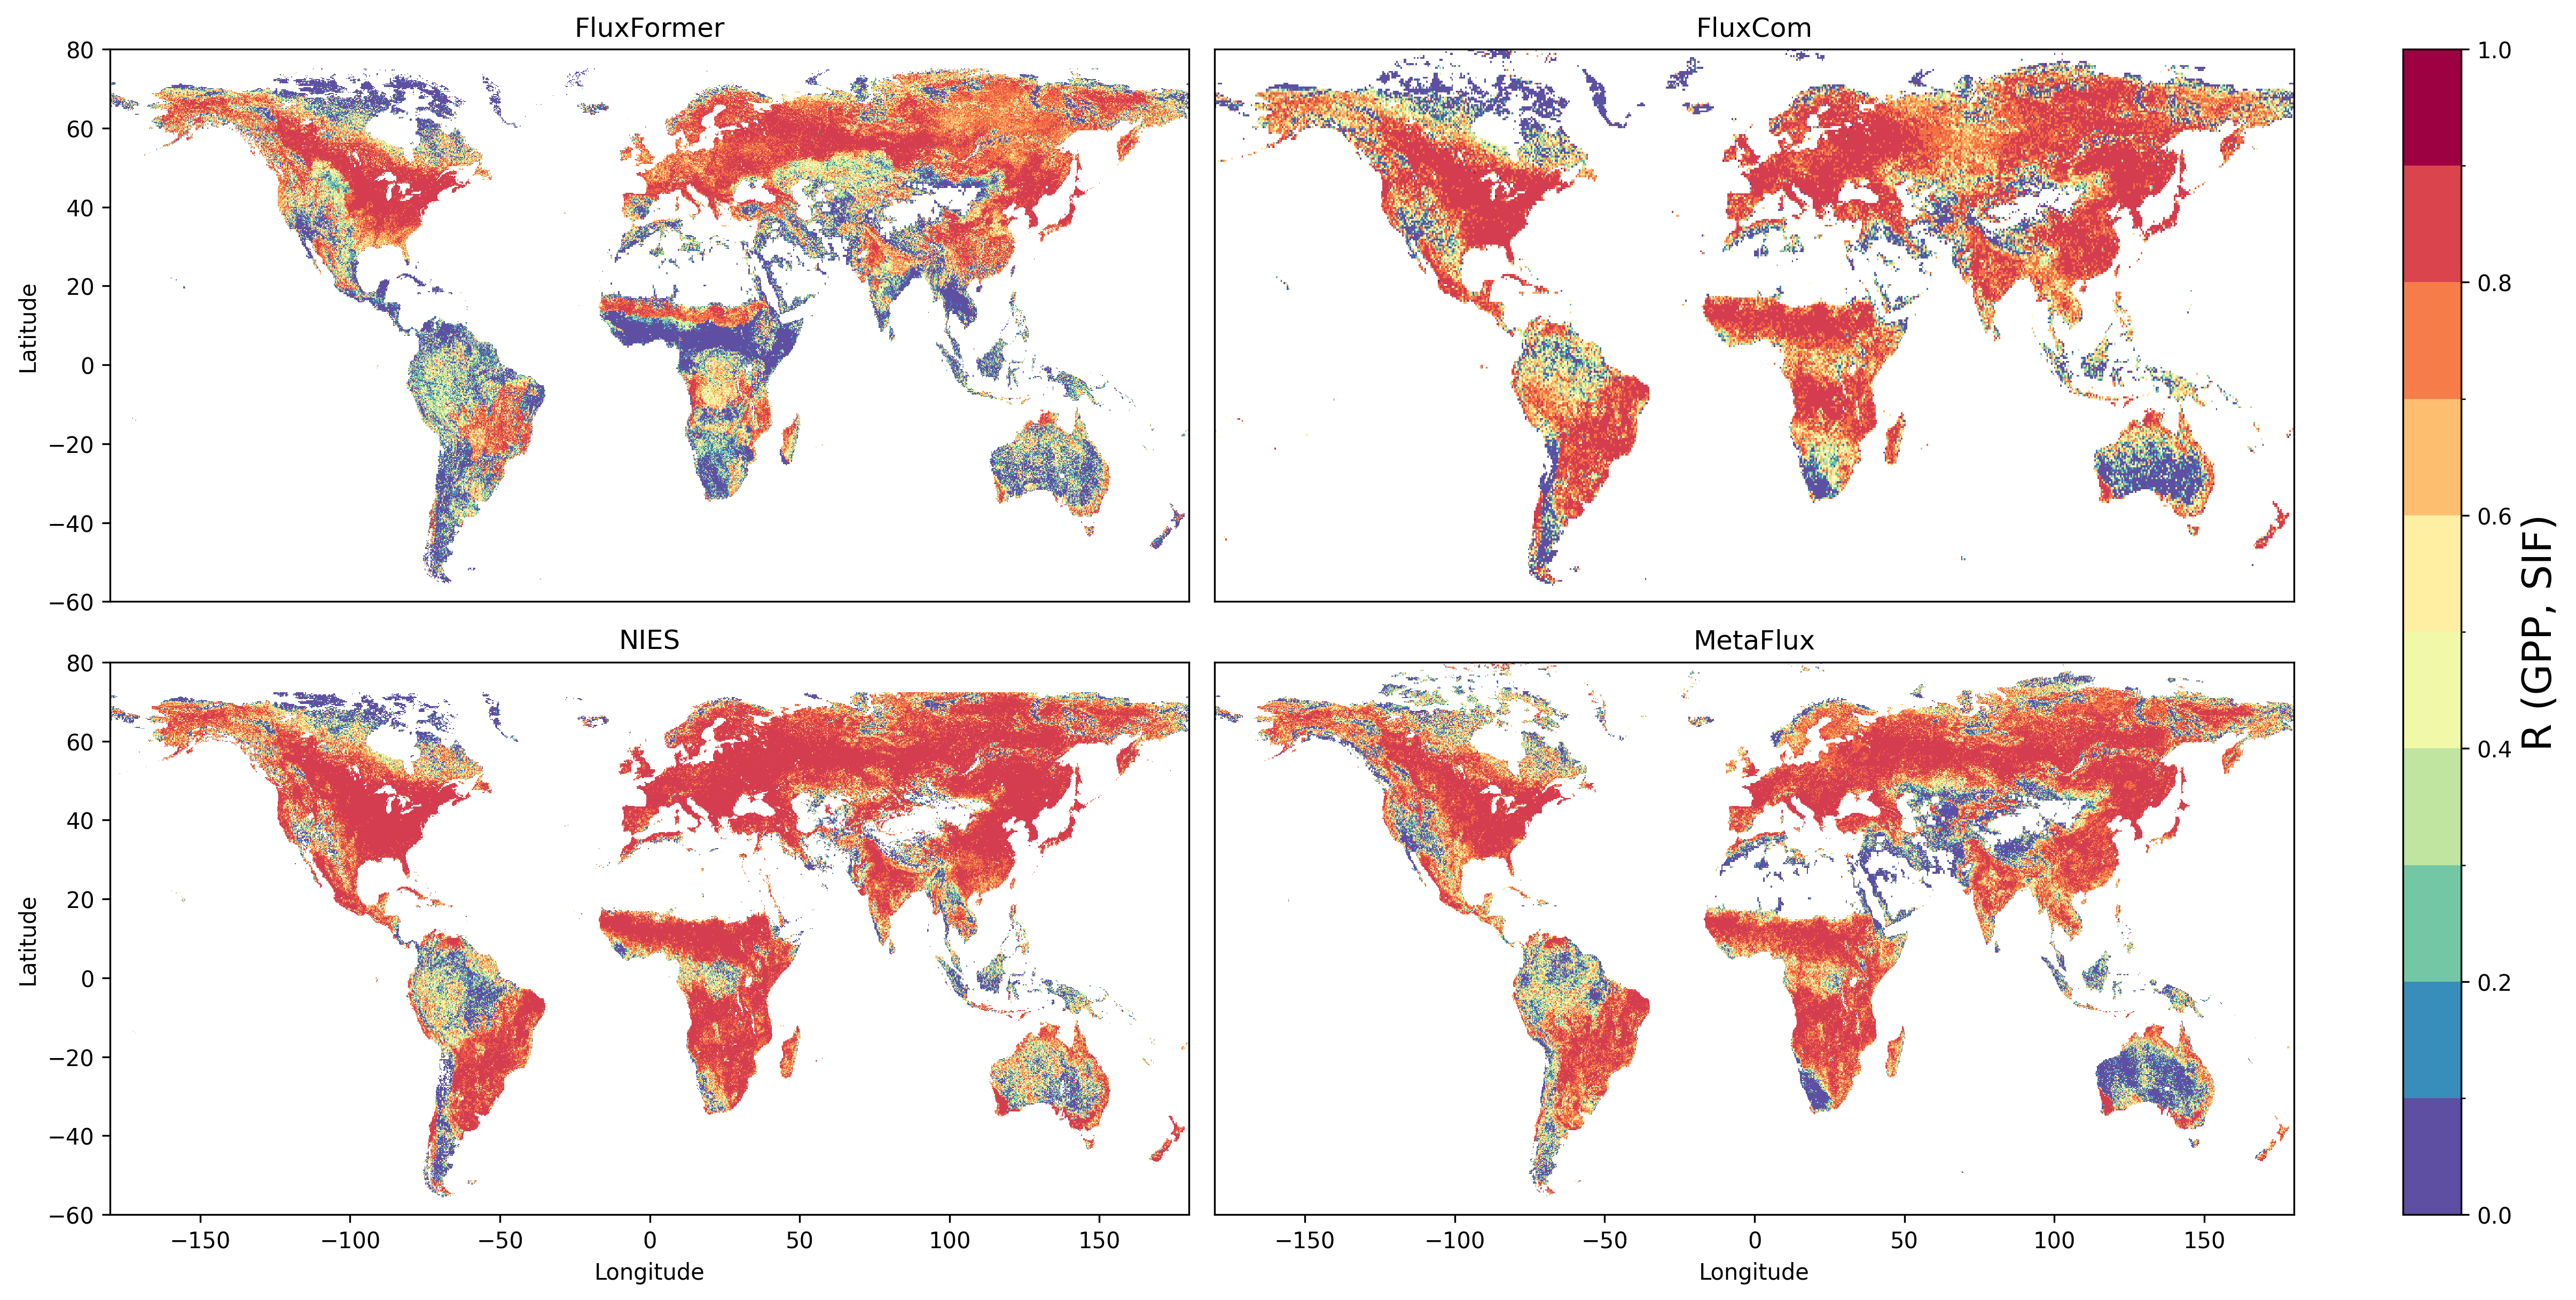
\includegraphics[width=\textwidth]{figs/chap6/val_TROPOMI_SIF.png}
      \caption{TROPOMI SIF}
      \label{fig:chap6_fig5b}
    \end{subfigure}
    \caption[Validation with SIF products]{Validation with SIF products: CSIF (a) TROPOMI SIF (b)}
    \label{fig:chap6_fig5}
\end{figure}

Previous studies generally assumed that linear relationship between GPP and SIF \citep{guanter2012retrieval, yang2017chlorophyll}. However this assumptions across climate regions and PFTs remains uncertains \citep{gu2019sun, xiao2019solar, zhang2016model, chen2021seasonal} especially in tropical regions where the evidents from showing that weak or no relationships of GPP with SIF in there as well as in South America and in subtropical Africa \citep{doughty2021global}.
The results are illustrated in Figure \ref{fig:chap6_fig5a} and Figure \ref{fig:chap6_fig5b}. We observed that our data exhibits lower correlation with CSIF and TROPOMI SIF in tropical regions (Central and South America, West and Central Africa, and Southeast Asia) and arid regions compared to FLUXCOM, NIES, and MetaFlux. This finding aligns with \citep{sanders2016spaceborne}, indicating weaker seasonality in these regions.\par


\subsubsection*{Interannual variations between products}
\paragraph*{Interannual trend}

The interannual trends of FluxFormer and other products (FLUXCOM, NIES, and MetaFlux) are illustrated in Figure \ref{fig:chap6_fig7a}. We examined the global annual time series from 2001 to 2019 to analyze the trend in Gross Primary Productivity (GPP). Our dataset exhibits the highest positive trend, with a growth rate of 0.45 PgC/year. The second-highest trend is observed in the NIES global annual time series, with a growth rate of 0.32 PgC/year. MetaFlux shows a small increasing trend, albeit with an insignificant p-value of 0.08. On the other hand, FLUXCOM indicates a small negative trend, with a reduction rate of 0.04 PgC per year.\par

Our long-term GPP trend aligns with the expected increase due to the CO\textsubscript{2} fertilization effect, anticipated to enhance the land carbon sink \citep{piao2020characteristics, guo2023estimating, yang2022divergent}.\par
\begin{figure}[tbh!]
    \centering
    \begin{subfigure}{\textwidth}
      \centering
      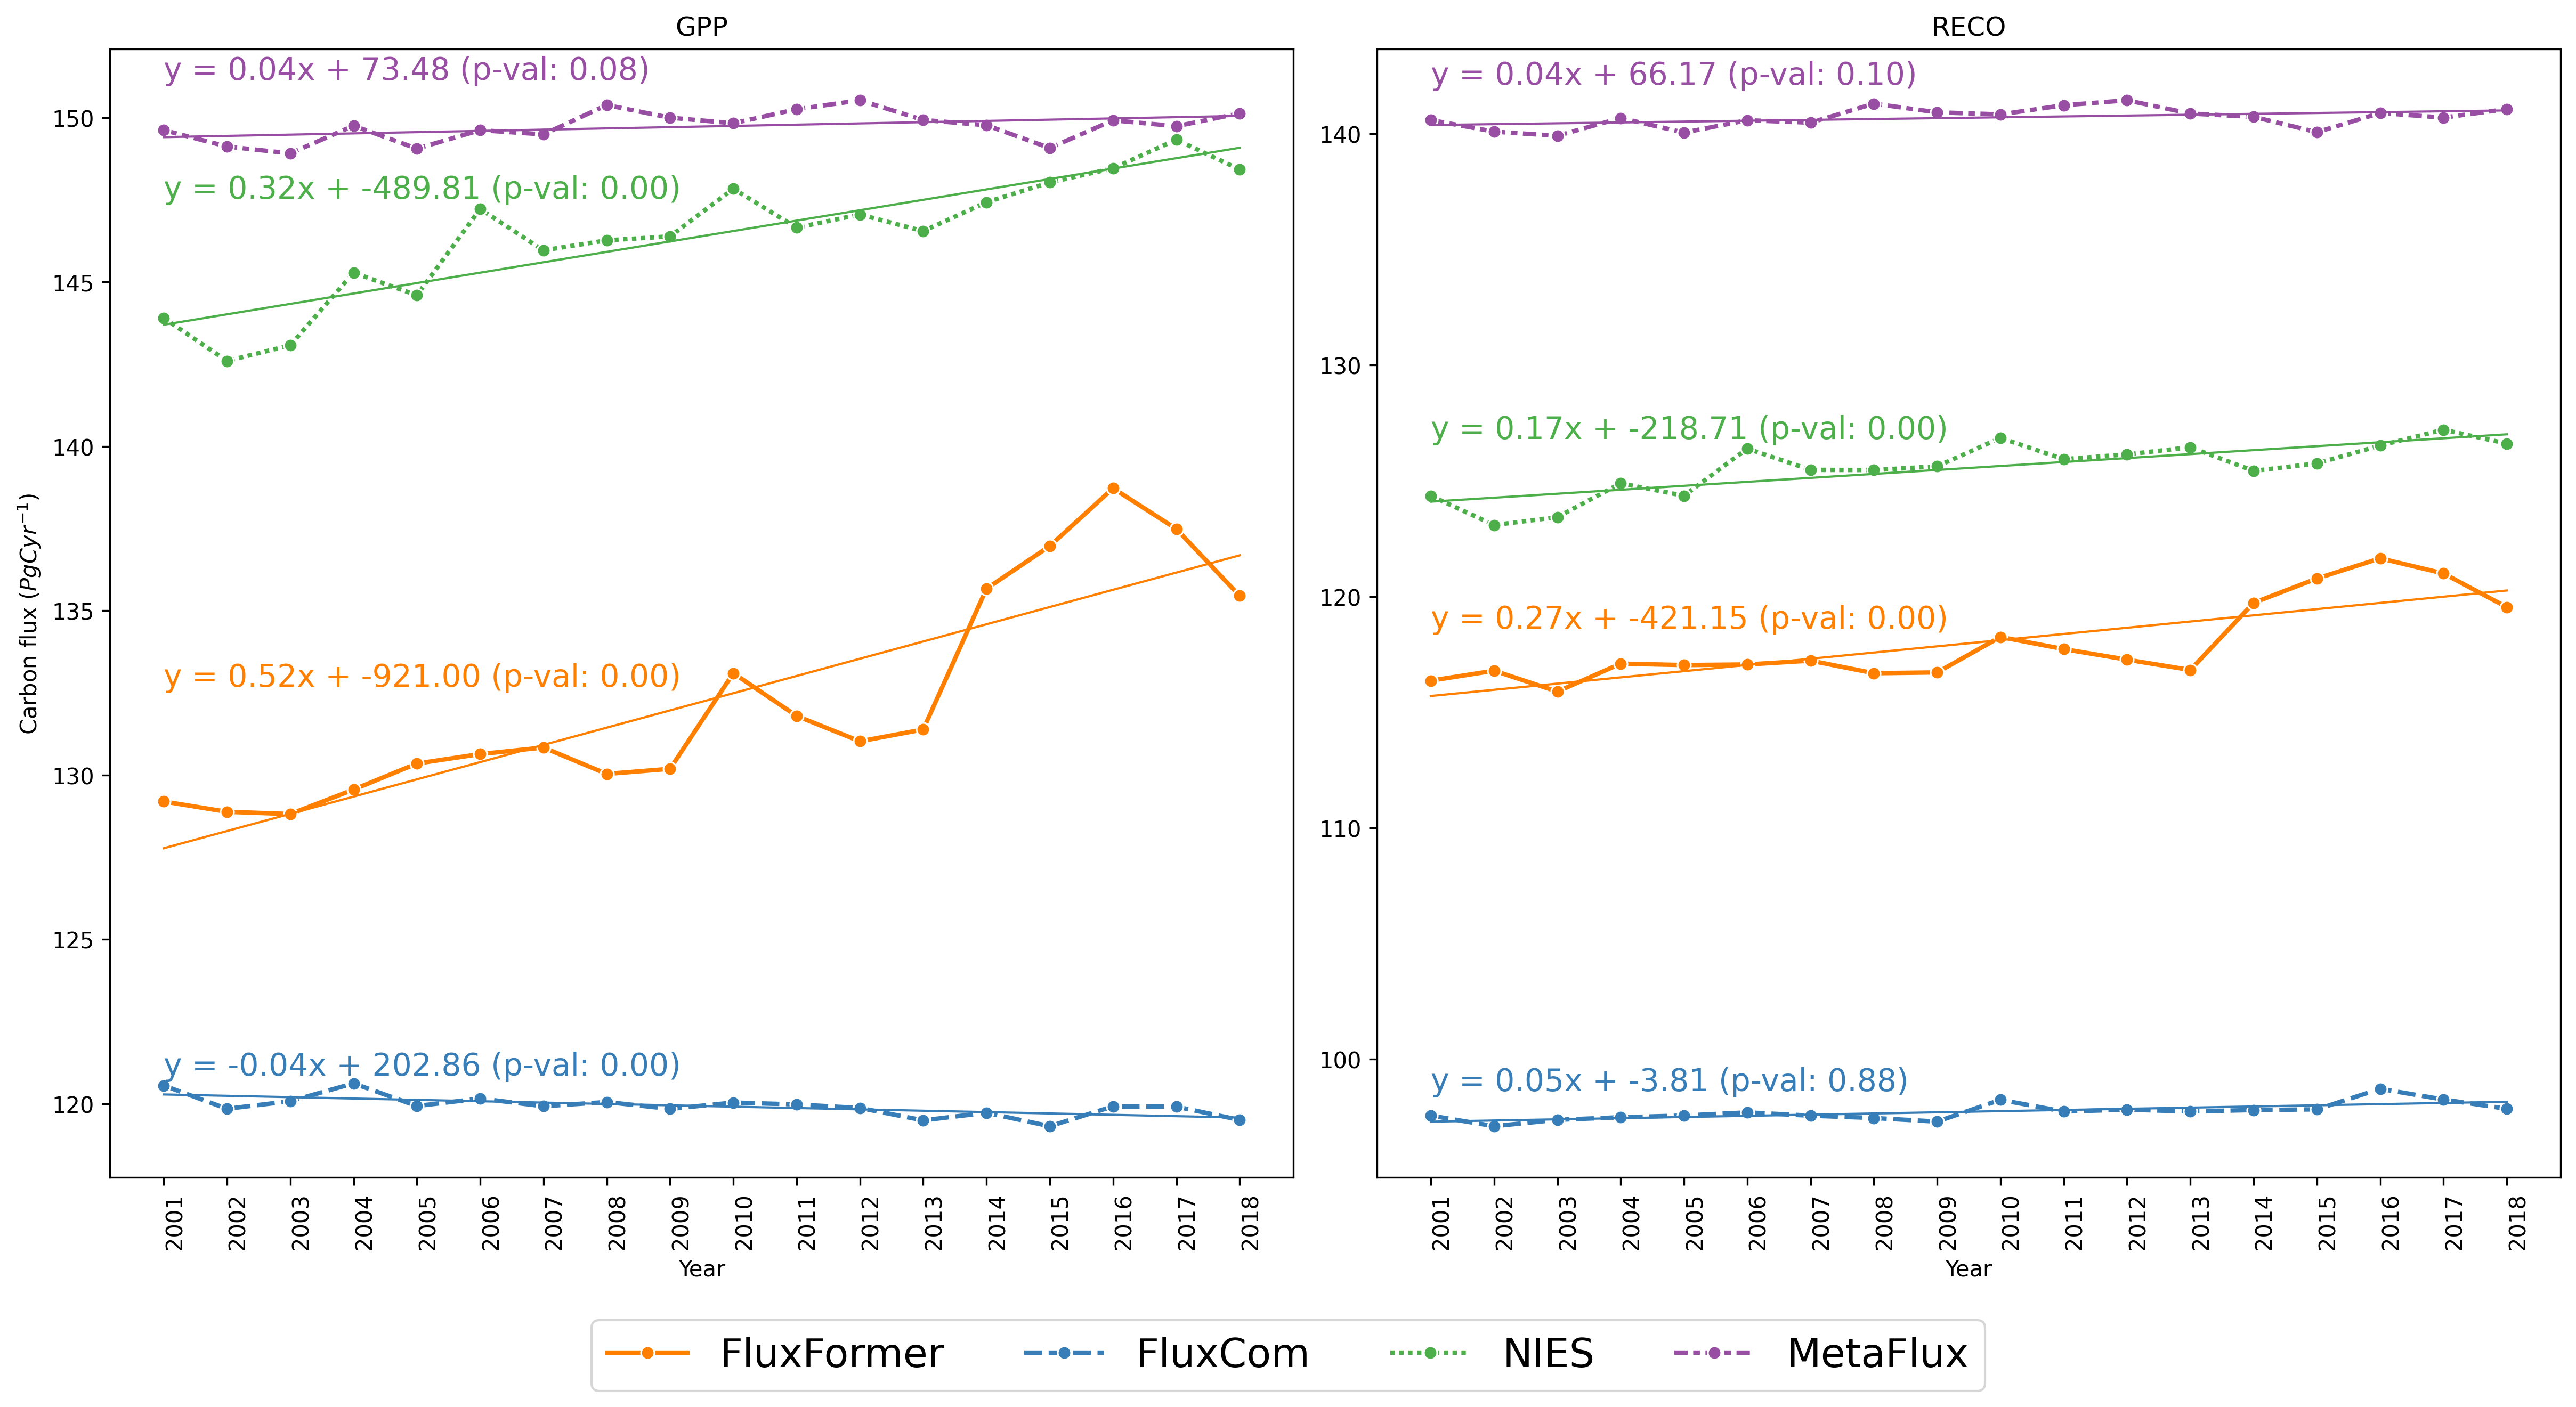
\includegraphics[width=\textwidth]{figs/chap6/global_annual_timeseries.png}
      \caption{Long term trend of global annual mean GPP and RECO from 2001 to 2019}
      \label{fig:chap6_fig7a}
    \end{subfigure}

    \begin{subfigure}{\textwidth}
      \centering
      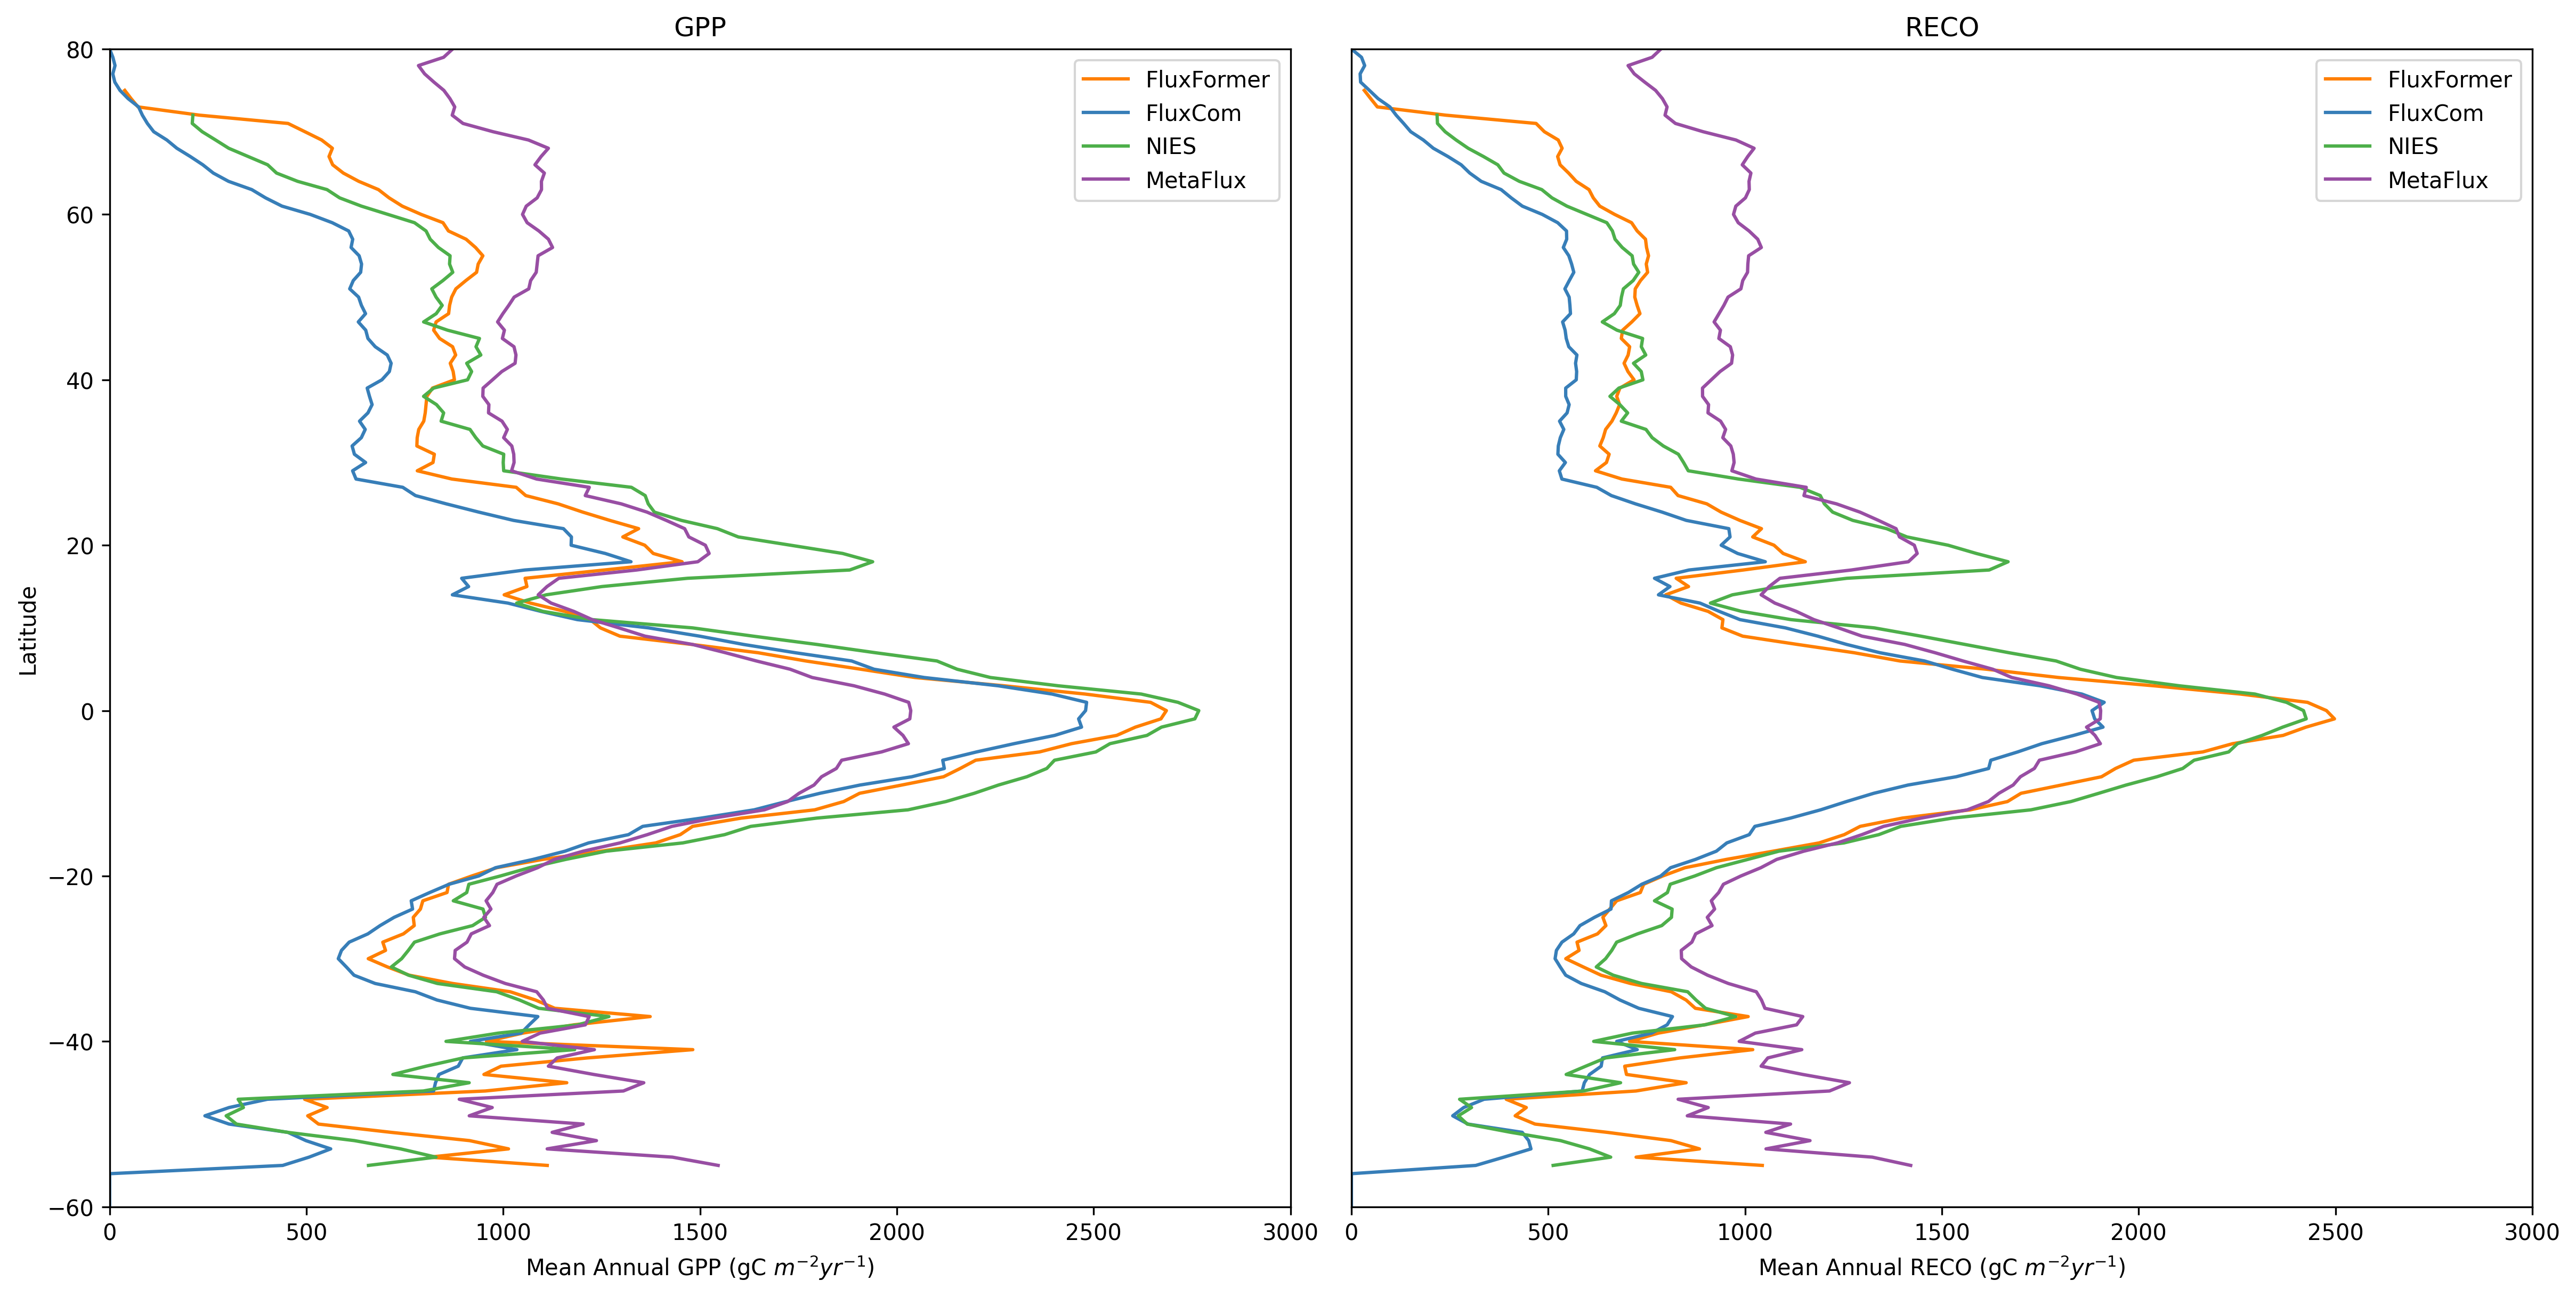
\includegraphics[width=\textwidth]{figs/chap6/lat_mean.png}
      \caption{Latitudinal distribution of GPP and RECO}
      \label{fig:chap6_fig7b}
    \end{subfigure}
    \caption[Long term trend and latitudinal distribution of GPP and RECO]{ (a) Long term trend and (b) latitudinal distribution of GPP and RECO}
    \label{fig:chap6_fig7}
\end{figure}

We also inspect the latitudinal distribution of GPP and RECO as depicted in Figure \ref{fig:chap6_fig7b}. All four products exhibit a gradual increase in both GPP and RECO values from cold climate regions to warm and humid climates in temperate and tropical regions. \par
\paragraph*{Interannual variations}
Finally, we assess the interannual variations of Gross Primary Productivity (GPP) and Ecosystem Respiration (RECO), as illustrated in Figures \ref{fig:chap6_fig8a} and \ref{fig:chap6_fig8b}, respectively. We observe that our data exhibits lower interannual variability than NIES in desert regions, including Australia, Central Asia, Central America, and South America. We posit that our data may be more reasonable, considering that in desert areas, GPP is expected to be extremely low \citep{hadley1981productivity}. Additionally, our dataset demonstrates smaller interannual variability than NIES in the northern parts of Eurasia and North America. \par
Our dataset displays greater interannual variability compared to FLUXCOM and MetaFlux. This difference could be attributed to the use of distinct remote sensing data sources for upscaling carbon fluxes. Specifically, we employed LAI and FAPAR from SPOT/VEGETATION and PROBA-V, which aligns with the approach described in \citep{zeng2020global}. In contrast, FLUXCOM and MetaFlux utilize input remote sensing data sourced from MODIS \citep{jung2019fluxcom, nathaniel2023metaflux}. \par
\begin{figure}[tbh!]
    \centering
    \begin{subfigure}{\textwidth}
      \centering
      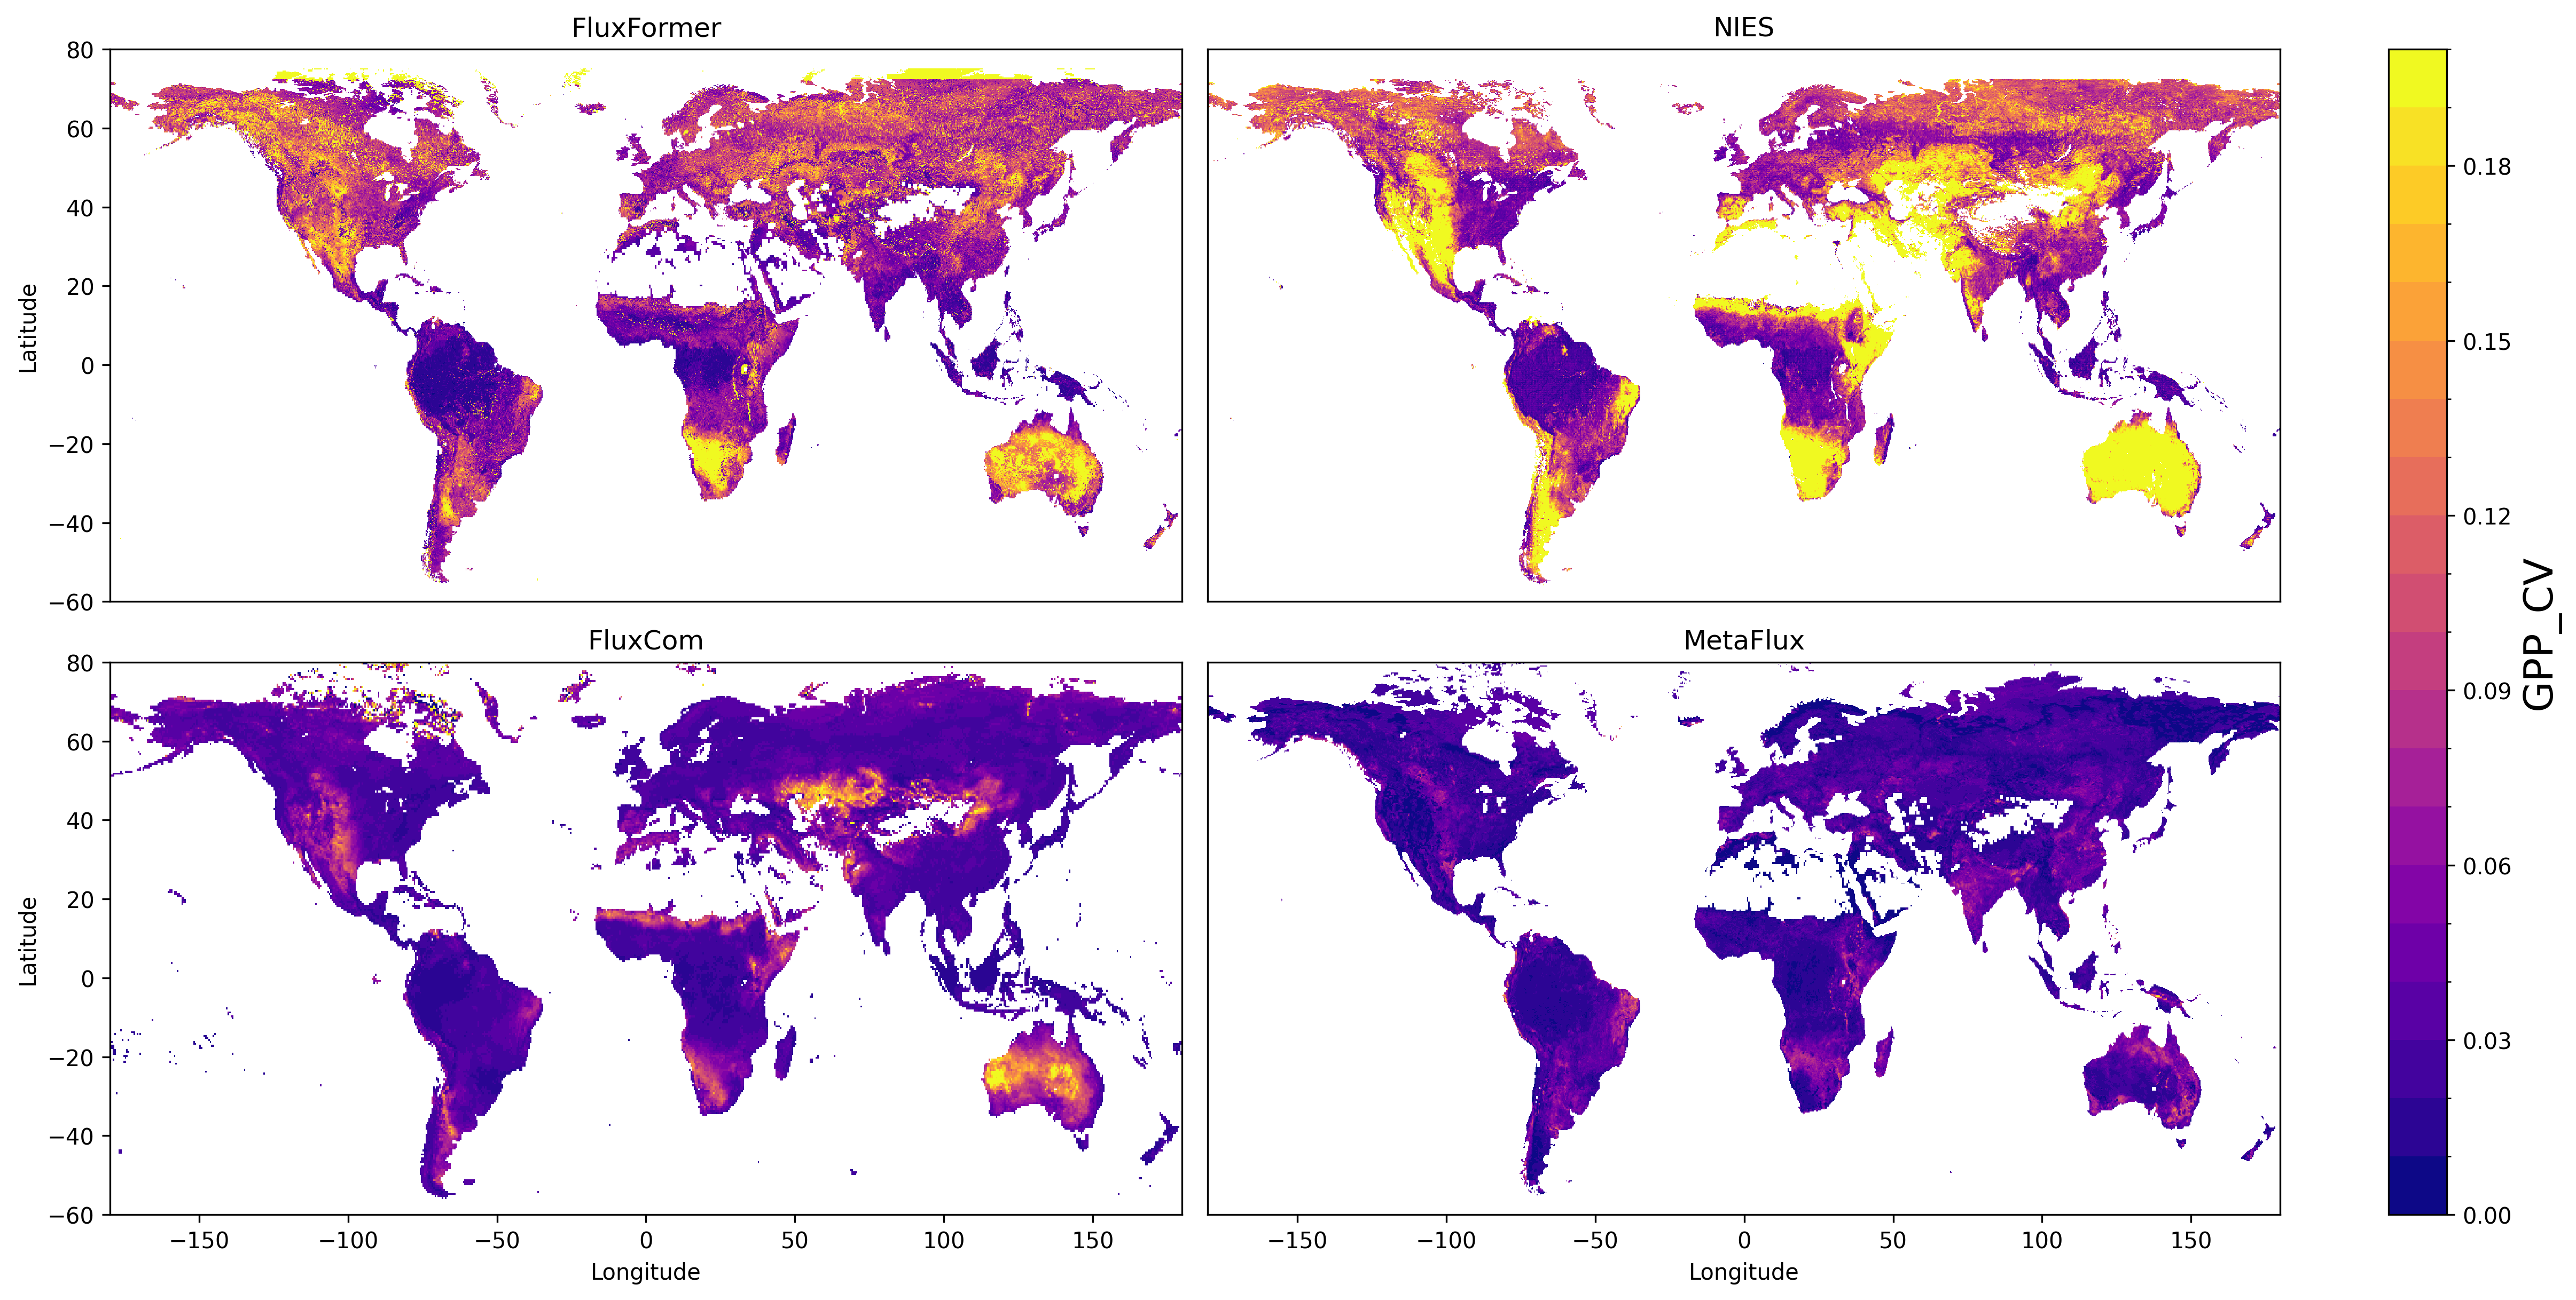
\includegraphics[width=\textwidth]{figs/chap6/IAV_GPP.png}
      \caption{GPP}
      \label{fig:chap6_fig8a}
    \end{subfigure}

    \begin{subfigure}{\textwidth}
      \centering
      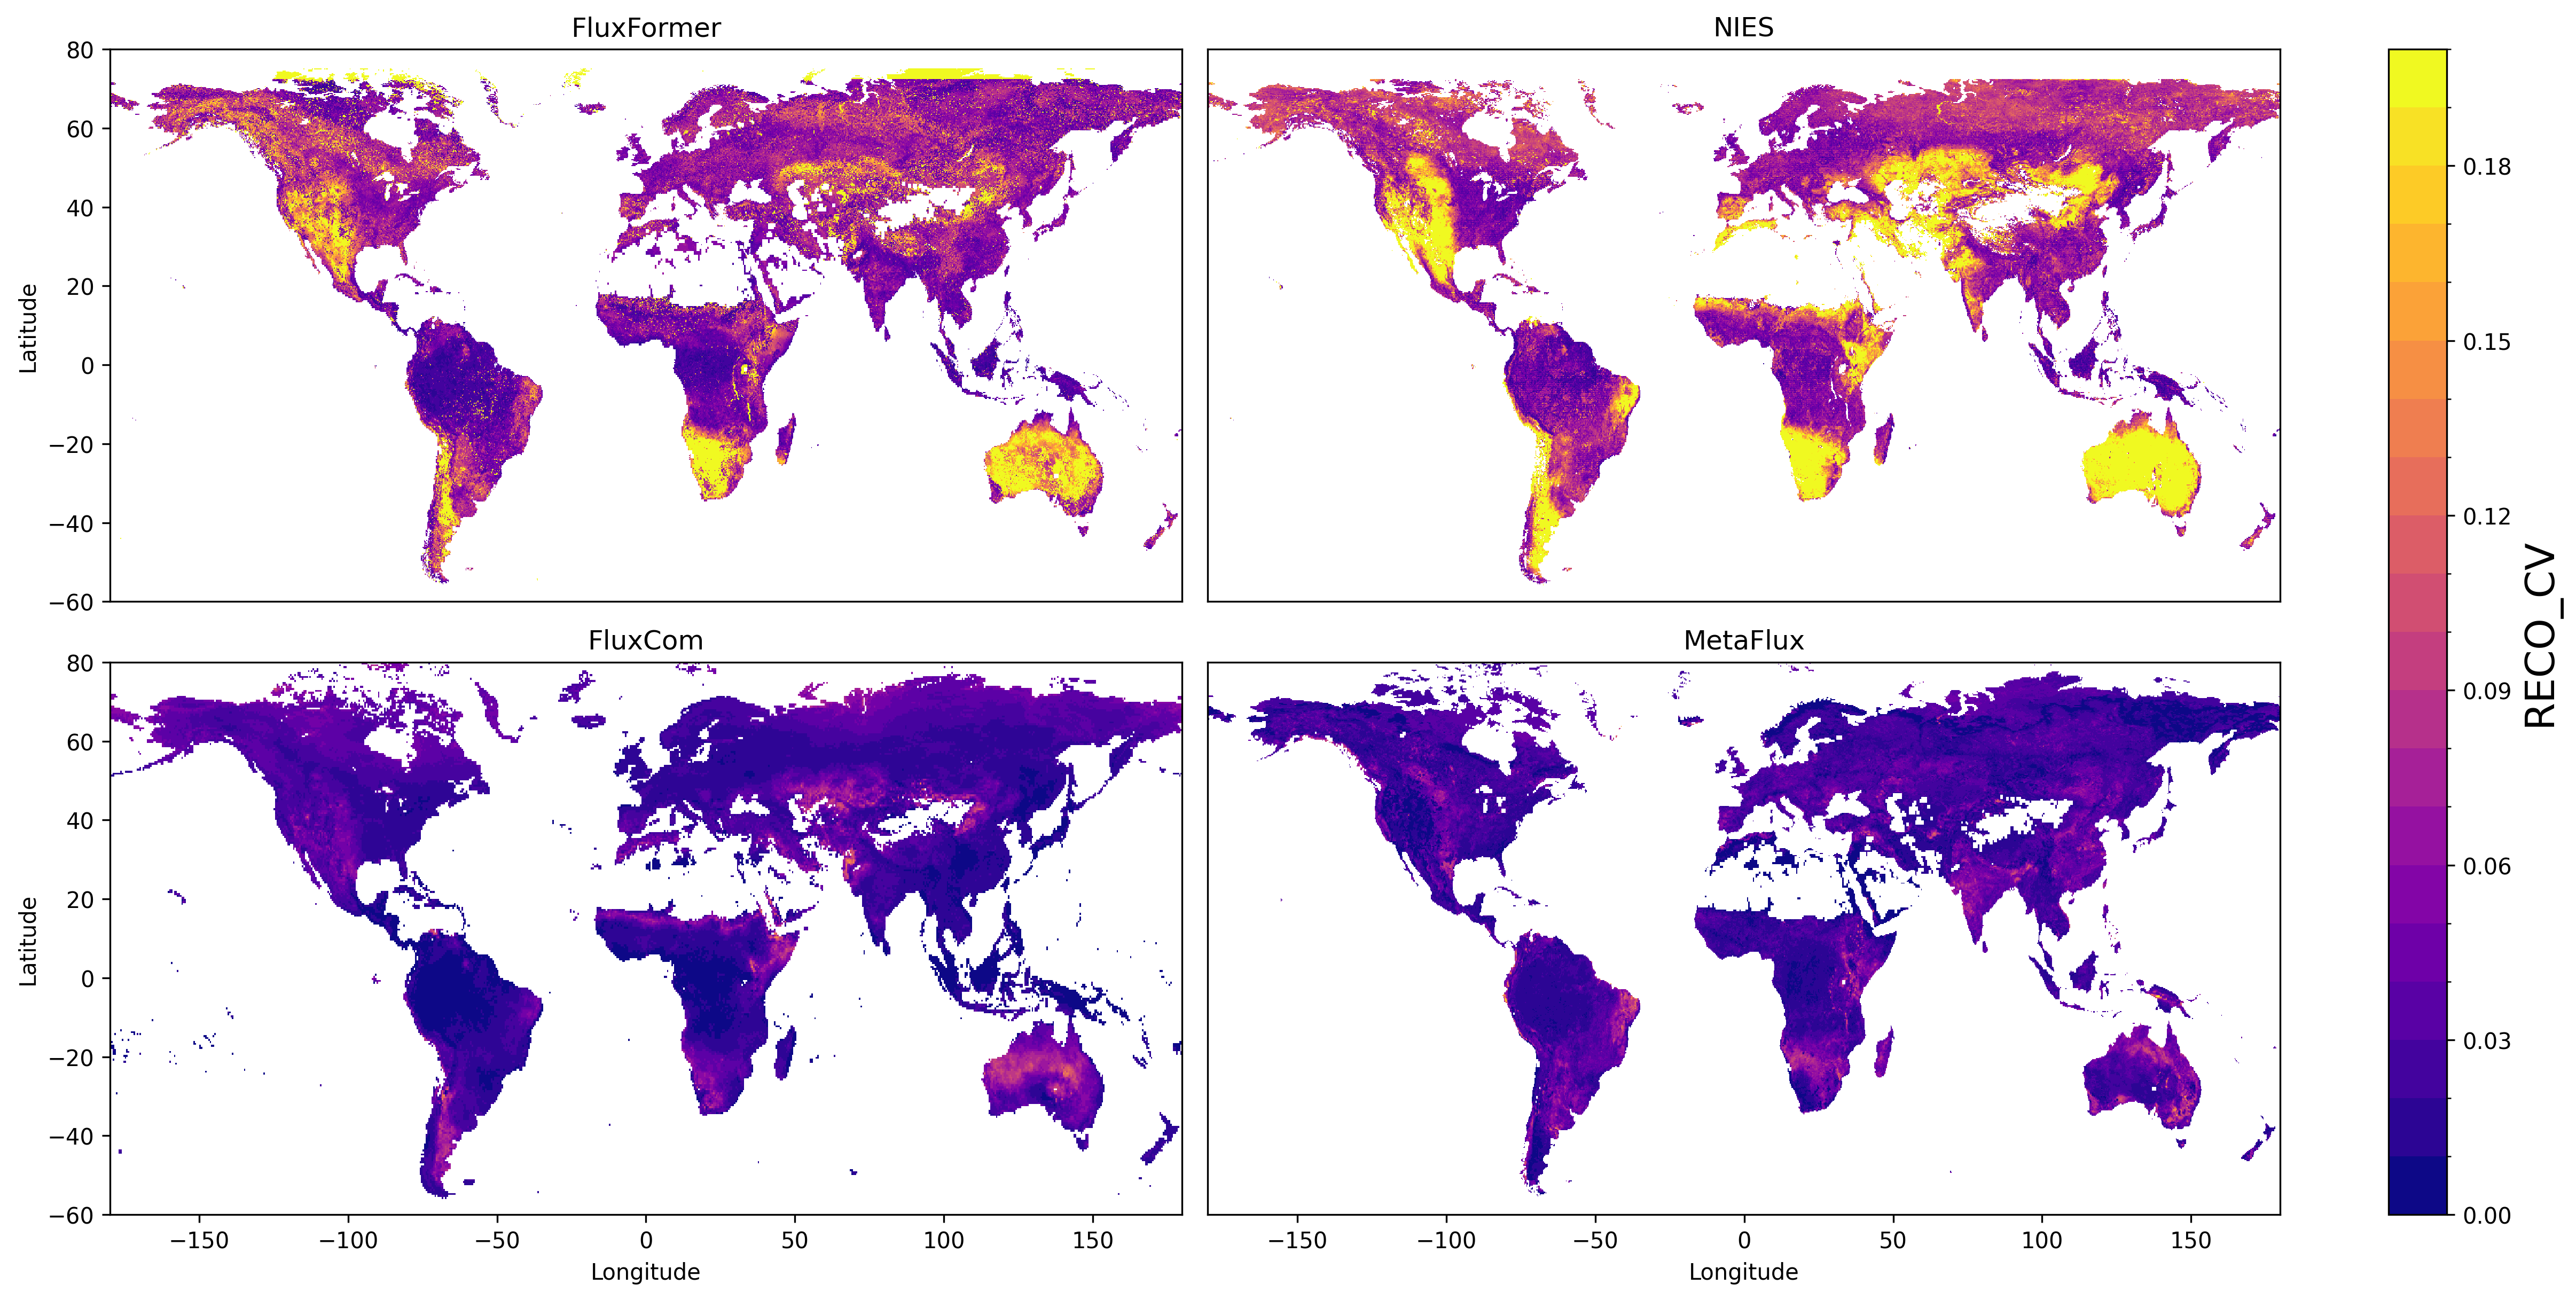
\includegraphics[width=\textwidth]{figs/chap6/IAV_RECO.png}
      \caption{RECO}
      \label{fig:chap6_fig8b}
    \end{subfigure}
    \caption{Interannual variations: GPP (a) RECO (b)}
    \label{fig:chap6_fig8}
\end{figure}
\subsection{Conclusion}
In this chapter, we present our work in upscaling global gross primary production and ecosystem respiration. This is achieved through the application of a multivariate timeseries transformer \citep{zerveas2021transformer} in conjunction with updated plant functional types data \citep{harper202229}. We provide monthly global data for GPP and RECO at a spatial resolution of 0.25° × 0.25°, covering the period from 1990 to 2019. \par

Our data shows improvement with increased correlation and reduced error when compared to FLUXNET 2015 data at both the site level and seasonal trends, outperforming FLUXCOM, NIES, and MetaFlux datasets. Particularly noteworthy is our data's strong correlation with the GPP seasonal trend in the tropical monsoon region ($R=0.84$), whereas FLUXCOM and MetaFlux exhibit no correlation with the ground measurements seasonal trend in that area. \par

We further assess the seasonal trend of our dataset using two SIF products, CSIF and TROPOMI SIF. Our dataset exhibits a strong correlation in cold and temperate regions, consistent with other datasets. However, in tropical and semi-arid regions, our dataset shows a lower correlation compared to others, a finding in line with \citep{sanders2016spaceborne}. This lower correlation is attributed to the weak seasonality of GPP in tropical regions and the high complexity of PFTs \citep{montgomery2001forest}, making the linear relationship less evident. \par

We also investigated the long-term trends of GPP and RECO from 2001 to 2019 and observed that our data exhibits the highest positive trend in GPP during this period, with a growth rate of 0.45 PgC per year. This finding aligns with studies such as \citep{{piao2020characteristics, guo2023estimating, yang2022divergent}}, supporting the assumption that the CO\textsubscript{2} fertilization effect should increase GPP over time. In contrast, MetaFlux and the widely used product FLUXCOM fail to replicate the long-term trend of GPP, contradicting the currently recognized significant greening observed from regional to global scales \citep{piao2020characteristics}. \par

Lastly, we scrutinize the interannual variations of our products in comparison with other datasets. We note that our dataset exhibits lower variations in extreme-low-GPP regions, such as deserts and semi-arid regions, when utilizing the same source of remote sensing data as NIES. However, our dataset shows higher variations than FLUXCOM and MetaFlux, possibly attributable to the utilization of different remote sensing resources. \par